\documentclass[12pt,a4paper]{article}
%packages
\usepackage[utf8]{inputenc}
\usepackage{amsmath}
\usepackage{amsfonts}
\usepackage{amssymb}
\usepackage{amsthm}
\usepackage{physics}
\usepackage{tikz-cd}
\usepackage{mathtools} % for text over and under iff etc, underset, underbrace etc

\usepackage{chngcntr}
\counterwithout{subsection}{section}
\setcounter{subsection}{-1}

\title{MT543 Topics in Algebra}
\author{Notes taken by Stephen Nulty and John Brennan}
\renewcommand{\abstractname}{Note:} 

%new commands
\newcommand{\zZ}{\ensuremath{\mathbb{Z}\,}}
\newcommand{\rR}{\ensuremath{\mathbb{R}\,}}
\newcommand{\cC}{\ensuremath{\mathbb{C}\,}}
\newcommand{\hH}{\ensuremath{\mathbb{H}\,}}
\newcommand{\fF}{\ensuremath{\mathbb{F}\,}}
\newcommand{\qQ}{\ensuremath{a+bi+cj+dk\,}}
\newcommand{\nn}{\ensuremath{n \times n\,}}
\newcommand{\xonen}{\ensuremath{(x_1,x_2,\ldots, x_n)\,}}
\newcommand{\xonem}{\ensuremath{(x_1,x_2,\ldots, x_m)\,}}

\newcommand{\cinf}{\ensuremath{C^{\infty}\,}}
\newcommand{\cinfm}{\ensuremath{C^{\infty}(M)\,}}
\newcommand{\cinfn}[1]{\ensuremath{C^{\infty}(#1)\,}}
\newcommand{\tpm}{\ensuremath{T_p M}}
\newcommand{\tm}{\ensuremath{T M}}
\newcommand{\tn}[1]{\ensuremath{T {#1}}}
\newcommand{\tqn}[2]{\ensuremath{T_{#1} {#2}}}
\newcommand{\dfp}{\ensuremath{df_p \,}}
\newcommand{\dfq}[1]{\ensuremath{df_{#1}\,}}
\newcommand{\df}{\ensuremath{df}}

\newcommand{\mnr}{\ensuremath{M_n(\rR)\,}}
\newcommand{\mnc}{\ensuremath{M_n(\cC)\,}}
\newcommand{\mnh}{\ensuremath{M_n(\hH)\,}}
\newcommand{\mnf}{\ensuremath{M_n(\fF)\,}}
\newcommand{\mr}[1]{\ensuremath{M_{#1}(\rR)\,}}
\newcommand{\mc}[1]{\ensuremath{M_{#1}(\cC)\,}}
\newcommand{\mh}[1]{\ensuremath{M_{#1}(\hH)\,}}
\newcommand{\glnr}{\ensuremath{GL_n(\rR)\,}}
\newcommand{\glnc}{\ensuremath{GL_n(\cC)\,}}
\newcommand{\glnh}{\ensuremath{GL_n(\hH)\,}}
\newcommand{\glnff}{\ensuremath{GL_n(\fF)\,}}
\newcommand{\glnf}{\ensuremath{GL_n(\fF^n)\,}}
\newcommand{\glr}[1]{\ensuremath{GL_{#1}(\rR)\,}}
\newcommand{\glc}[1]{\ensuremath{GL_{#1}(\cC)\,}}
\newcommand{\glh}[1]{\ensuremath{GL_{#1}(\hH)\,}}

\newcommand{\gon}{\ensuremath{O(n)\,}}
\newcommand{\gun}{\ensuremath{U(n)\,}}
\newcommand{\gspn}{\ensuremath{Sp(n)\,}}
\newcommand{\gok}[1]{\ensuremath{O(#1)\,}}
\newcommand{\guk}[1]{\ensuremath{U(#1)\,}}
\newcommand{\gspk}[1]{\ensuremath{Sp(#1)\,}}

\newcommand{\gson}{\ensuremath{SO(n)\,}}
\newcommand{\gsun}{\ensuremath{SU(n)\,}}
\newcommand{\gsln}{\ensuremath{SL(n)\,}}
\newcommand{\gsok}[1]{\ensuremath{SO(#1)\,}}
\newcommand{\gsuk}[1]{\ensuremath{SU(#1)\,}}
\newcommand{\gslk}[1]{\ensuremath{SL(#1)\,}}

\newcommand{\sph}[1]{\ensuremath{S^{#1}}\,}
\newcommand{\tor}[1]{\ensuremath{T^{#1}}\,}
\newcommand{\rpk}[1]{\ensuremath{\mathbb{R}\mathrm{P}^{#1}}\,}

\newcommand{\ra}{\ensuremath{\Rightarrow}}
\newcommand{\la}{\ensuremath{\Leftarrow}}
\newcommand{\cin}{\ensuremath{\mathcal{I}_n\,}}
\newcommand{\ci}[1]{\ensuremath{\mathcal{I}_{#1}\,}}
\newcommand{\im}{\ensuremath{\operatorname{im}}}
\newcommand{\ol}[1]{\overline{#1}}
\newcommand{\ipm}[2]{\ensuremath{\left\langle #1, \, #2 \right\rangle}}
\newcommand{\ul}[1]{\underline{#1}}

\newcommand{\quot}[2]{\ensuremath{\;^{#1} / _{#2}\;}}

\newcommand{\bij}[1]{\ensuremath{\operatorname{Bij}(#1)}}
\newcommand{\homeo}[1]{\ensuremath{\operatorname{Homeo}(#1)}}
\newcommand{\diffeo}[1]{\ensuremath{\operatorname{Diffeo}(#1)}}
\newcommand{\isom}[1]{\ensuremath{\operatorname{Isom}(#1)}}
\newcommand{\jac}[1]{\ensuremath{\operatorname{Jac}{#1}}}

\newcommand{\genericA}{\ensuremath{\pmqty{a_{11} & \ldots & a_{1n} \\ \vdots & \vdots & \vdots \\ a_{n1} & \ldots & a_{nn}}}}

% vertical and horizontal bars for matrix columns and rows.
\newcommand*{\vertbar}{\rule[-1ex]{0.5pt}{2.5ex}}
\newcommand*{\horzbar}{\rule[.5ex]{2.5ex}{0.5pt}}

%proofs etc
\newtheorem{thm}{Theorem}[subsubsection]
\newtheorem{defn}[thm]{Definition}
\newtheorem{lemma}[thm]{Lemma}
\newtheorem{prop}[thm]{Proposition}
\newtheorem{obs}[thm]{Observation}
\newtheorem{cor}[thm]{Corollary}

%block matrices
\newcommand{\rvline}{\hspace*{-\arraycolsep}\vline\hspace*{-\arraycolsep}}
\newcommand{\bigzero}{\mbox{\normalfont\Large\bfseries 0}}
\newcommand{\bigld}{\mbox{\normalfont\Large\bfseries \ldots}}
\newcommand{\bigvd}{\mbox{\normalfont\Large\bfseries \vdots}}

\renewcommand{\thesubsection}{\arabic{subsection}}
\makeatletter
\def\@seccntformat#1{\@ifundefined{#1@cntformat}%
   {\csname the#1\endcsname\quad}%    default
   {\csname #1@cntformat\endcsname}}% enable individual control
\newcommand\section@cntformat{}     % section level 
\newcommand\subsection@cntformat{\thesubsection.\space} % subsection level
\newcommand\subsubsection@cntformat{\thesubsubsection.\space} % subsubsection level
\makeatother

\renewcommand{\thethm}{\arabic{subsection}.\arabic{subsubsection}.\arabic{thm}}

%begin
\begin{document}
\maketitle
\begin{abstract}
    Any transcription mistakes and typos are my own.
\end{abstract}
Lectures by David Wraith. Lie Groups and Lie Algebras.
\section{Lecture 1 25/09/23}
missed this lecture - some intro to do with spheres, transformations and symmetries and other motivational stuff. Definition of an algebra (bilinear product) over a field.

\subsection{Introduction}

Lie groups have a dual nature: they are groups but also very special topological spaces. The algebraic and topological (spatial) properties are closely aligned. Lie groups and Lie algebras lie at the intersection of algebra, topology, geometry, analysis and more.

\begin{defn}
An algebra is a vector space $V$ equipped with a bilinear map $m:V\times V \to V$.
\end{defn}

Note, the ``multiplication" map $m$ does not have to be commutative or associative. In general, Lie algebras are neither commutative nor associative. Recall,
\begin{align*}
&\mbox{Commutativity: } m(u, v) = m(v, u), \\
&\mbox{Associativity: } m(m(u, v), w) = m(u, m(v, w)).
\end{align*}
Every Lie group has an associated Lie algebra which encodes many properties of the group. Often this allows problems about Lie groups to be reduced to problems in (fancy!) linear algebra.

\subsection*{Example of a Lie group}

The set of rotations of a ball centred on $O$ in $\rR^3$ is a Lie group. It is a group under composition of rotations. To ``see" the topology here, notice that it makes sense to talk about two rotations being ``close", so there is a sense of space. It makes sense to consider a continuous family of rotations. Continuity implies the existence of topology. We can identify this group with the matrix group $SO(3)$. The map $\rR^3 \to \rR^3$ given by $x \mapsto Ax$ for $A \in SO(3)$ is a rotation and every rotation occurs in this way. $SO(3)$ is a subset (but not a subgroup) of the set/group of all $(3\times 3)$-real matrices $M_3(\rR)$. By listing the elements of any $3\times 3$ matrix we get a bijection $M_3(\rR) \to \rR^9$. As $\rR^9$ has a natural topology (metric), this gives a natural topology on $M_3(\rR)$ and by restriction on $SO(3)$.


\section{Lecture 2 27/09/23}
Sorting out tutorial times. Lectures: Monday 2pm MS2, Wednesday 2pm LGH, Thursday 12pm MS2.

Lie Groups, dual nature, Groups but also a topological geometrical character. Can prove things with a mix of both methods - intersection of various areas.

\subsection{Groups of matrices}
\subsubsection{General Linear Groups}

Quaternions will have a central role.

Consider groups of $N\times N$ matrices over the fields \rR and \cC and also over the quaternions.

\begin{defn}
The quaternions \hH is a 4-dim real vector space with standard basis elements $1,i,j,k$, equipped with an associative linear multiplication operation defined by

\[i^2=j^2=k^2=-1, \quad ij=k, jk=i, ki=j\]
\end{defn}

So a generic quaternion takes the form $a+bi+cj+dk$, $a,b,c,d \in \rR$.

Observe, $ji=j(jk)=(jj)k$ (by associativity) $=j^2k=-k$. Similarly $kj=-i$ and $ik=-j$.

e.g. $(2+i-3k)(5+2i-j+k)=10+4i-2j+2k+5i-2-k-j-15k-6j-61+3$ etc.

Quaternions is not commutative, so is not a field. However it is a skew field (division algebra).

Terminology - In $a+bi+cj+dk$, $a$ is called the real or scalar part, and the rest $bi+cj+dk$ imaginary or vector part.

In analogy with complex numbers,

\begin{defn} 
1. The conjugate of  \qQ , is $\overline{\qQ}=a-bi-cj-dk$
2. The norm of \qQ is  $|\qQ |=\sqrt{a^2+b^2+c^2+d^2}$
\end{defn}

Thus \hH is a normed vector space. Next observe that for each $q\in\hH$ $q\bar{q}=\bar{q}q = |q|^2$.

therefore (symbol) $q^{-1}=\bar{q}/|q|^2$. So $qq^{-1}=q\bar{q}/|q|^2=|q|^2=1$, similarly for $q^{-1}q=1$.

This allows division $q_1\cdot q_2^{-1}=q_1 \bar{q_2}/|q_2|^2$. Writing $q_1/q_2$ is ambiguous however. $q_1 q_2^{-1}\neq q_2^{-1} q_1$ generically.

Clearly $\rR \subset \cC \subset \hH$. A classic theorem of Frobenius asserts that \rR, \cC, \hH are the only real associative division algebras. These objects similarly play a distinguished role in Lie group theory.

Convention: Suppose V is a vector space over the quaternions \hH. We will adopt the convention that whenever we scale a vector $v\in V$ by a scalar $\lambda \in \hH$, we multiply on the left, i.e. $\lambda v$

Let $M_n(\rR),  M_n(\cC),  M_n(\hH)$ denote the sets (vector spaces!) of all $n\times n$ matrices over $\rR, \cC,  \hH$.

\begin{defn} 
The General Linear Groups $GL_n(\rR)$, resp. $GL_n(\cC)$ is the group of  $n\times n$ invertible matrices with \rR resp \cC coefficients. (Group under multiplication). Equivalently $GL_n(\rR)=\{A\in M_n(\rR)| \det(A)\neq0\}$. Similarly $GL_n(\cC)=\{A\in M_n(\cC)| \det(A)\neq0\}$.
\end{defn}

(return to the idea of determinants of quaternions later).

Recall that for any matrix $A\in\mnr$ we have two associated linear maps $L_A:\rR^n\to \rR^n, L_a(\vec{x})=A\vec{x},$  $R_A:\rR^n\to \rR^n, R_a(\vec{x})=\vec{x}A.$ 

It is well know that $A$ is invertible (RC cases) $\iff$ $\det(A)\neq0$ $\iff$ $L_A, R_A$ are isomorphisms.

\section{Lecture 3 02/10/23}
Thursday lecture moved to Friday at 10am in MS2.

Reminder: 
\begin{itemize}
\item Quaternions \hH, multiplication is associative not commutative. If $V$ is a \hH - vector space, we scale from the left only, i.e. $\lambda v$ for $\lambda \in \hH, v\in V$. 
\item General linear groups \glnr, \glnc groups under $*$ of all invertible \rR resp. \cC \nn - matrices.
\item $A\in \mnr, \mnc$ is invertible iff $\det A \neq 0$ iff $L_A, R_A$ are both invertible where $L_a(\vec{x})=A\vec{x}$, $R_a(\vec{x})=\vec{x}A.$ 
\end{itemize}

We now consider \mnh.

\begin{defn}
A function $f:\hH ^n \to \hH^n$ is \hH - linear if  $f ( \lambda _1 v_1+\lambda _2 v_2)=\lambda _1 f(v_1)+\lambda _2 f(v_2),\; \forall \lambda _1 \lambda _2 \in \hH , v_1,v_2 \in \hH ^n$.
\end{defn}

\begin{lemma}
For $A \in \mnh$, $R_A:\hH^n\to \hH^n$ given by $R_a(\vec{x})=\vec{x}A$  for $v\in \hH^n$ a row vector, is \hH - linear, however $L_A$ is in general not \hH - linear.
Proof: exercise
\end{lemma}

idea is that associativity makes $\lambda v A$ ok, but not with left multiplication which is interfered by commutativity.

\begin{lemma}
For $A \in \mnh$, $R_A:\hH^n\to \hH^n$, is an \hH - linear isomorphism iff $A$ is invertible, i.e. $\exists B\in \mnh$ such that $AB=BA=I_n$.
\end{lemma}

\begin{proof}
($\ra$) If $R_A$ is an iso. then there is a \hH -linear inverse $(R_A)^{-1}: \hH ^n \to \hH ^n $. There is a corresponding matrix $B\in \mnh$. Since $R_A \circ (R_A)^{-1}=R_A \circ (R_A)^{-1}=I_n$. we deduce $BA=AB=I_n$ (NB order of matrices here!). Therefore $B=A^{-1}$.

($\la$) Similar.
\end{proof}

\begin{defn}
The quaternionic general linear group $\glnh = \{A\in \mnh | A \text{ is invertible}\} = \{A\in \mnh| R_a \text{ is an iso.}\}$
\end{defn}

NB: There is a problem with the notion of \hH - determinant due to non-commutativity we'll return to this later (possible to define determinant and \glnh as ones with non-zero determinant, but defining it requires some thought.)

It turns out that we can view \cC and \hH- matrices/linear maps in terms of \rR- matrices. 

\begin{prop}
There is a real linear map $\rho_n: \mnc \to \mr{2n}$ such that the following diagram commutes. 
\begin{center}
\begin{tikzcd}
  \cC^n \arrow{d}{R_A} \arrow{r}{\theta_n}
    & \rR^{2n} \arrow{d}{R_{\rho_n(A)}} \\
  \cC^n \arrow{r}{\theta_n}
&\rR^{2n} \end{tikzcd}
\end{center}
where $\theta _n : \cC ^n \to \rR ^{2n}$ is given by $\theta _n (a_1+ib_1, \ldots , a_n+ib_n )=(a_1,b_1,\ldots, a_n,b_n)$.
\end{prop}

(compactly every complex matrix can be viewed as a real matrix of twice the size)

Remark: $\theta _n $ is  a real linear isomorphism. This forces $R_{\rho _n (A)}=\theta _n \circ R_A \circ \theta _n^{-1}$.

This is linear and therefore there is a corresponding matrix $\in \mr{2n}$.

\begin{proof}
Given that $\theta _n$ is a real-linear isomorphism, consider the map $\theta_n \circ R_A \circ \theta_n^{-1} : \rR^{2n} \to \rR^{2n}$. This is clearly real-linear, and hence corresponds to some $(2n\times 2n)$-real matrix which depends on $A$. Call this matrix $\rho_n(A)$. Thus we obtain a map $\rho_n (A) : \mnc \to \mr{2n}$, and the requirement that $\theta_n \circ R_A = R_{\rho_n (A)} \circ \theta_n$ is automatrically satisfied by construction. 

It remains to show that $\rho_n$ is a real-linear map. To this end we compute for $A_1, A_2 \in \mnc$ and $\lambda, \mu \in \rR$:

\begin{align*}
R_{\rho_n (\lambda A_1 + \mu A_2)} 
&= \theta_n \circ R_{\lambda A_1 + \mu A_2} \circ \theta_n^{-1} \\
&= \theta_n \circ (\lambda R_{A_1} + \mu R_{A_2}) \circ \theta_n^{-1} \\
&= \lambda \theta_n \circ R_{A_1} \circ \theta_n^{-1} + 
   \mu     \theta_n \circ R_{A_2} \circ \theta_n^{-1} \\
&= \lambda R_{\rho_n(A_1)} + \mu R_{\rho_n(A_2)} \\
&= R_{\lambda \rho_n(A_1) + \mu \rho_n(A_2)}.\\
\end{align*}
As for any $X, Y \in \mr{2n}$ we have $R_X = R_Y$ if and only if $X = Y$, we deduce that $\rho_n (\lambda A_1 + \mu A_2) = \lambda \rho_n(A_1) + \mu \rho_n(A_2)$ as required.
\end{proof}

\begin{obs}
$\rho_n$ is injective. Proof: exercise.
\end{obs}

\begin{lemma}
$\rho _n$ satisfies $\rho_n(AB)= \rho_n(A)\rho_n(B)$.
\end{lemma}

Remark: When we take 1.1.10 together with 1.1.9 and 1.1.8, we see that $\rho_n$ is an injective real-algebra homomorphism.

\begin{proof}
We compose commutative squares from 1.1.8 to get

\begin{center}
\begin{tikzcd}
  \cC^n \arrow{d}{R_A} \arrow{r}{\theta_n}
    & \rR^{2n} \arrow{d}{R_{\rho_n(A)}} \\
  \cC^n \arrow{r}{\theta_n}  \arrow{d}{R_B}
&\rR^{2n} \arrow{d}{R_{\rho_n(B)}} \\
  \cC^n \arrow{r}{\theta_n}
&\rR^{2n} 

\end{tikzcd}
\end{center}

On L.H.S. we have $R_B \circ R_A = R_{AB}$. (note order)

On R.H.S we have $R_{\rho_n(B)} \circ R_{\rho_n(A)} =R_{\rho_n(A)\rho_n(B)}$.

But since LHS is $R_{AB}$ this means $R_{\rho_n(AB)}= \text{composition on RHS}=R_{\rho_n(A)\rho_n(B)}$.
\end{proof}

It's not surjective however. Q: What exactly is $\rho_n(A)$? Consider $(a+ib)\in \mc{1}$. 

\[R_{(a+ib)}(x+iy)=(x+iy)(a+ib)=(ax-by)+i(ay+bx)\]

Now $\theta_1(x+iy)=(x,y) \in \rR^2$ etc.

So $\theta_1((ax-by)+i(ay+bx))=(ax-by,ay+bx)$

The corresponding map from $\rR ^2\to \rR^2$ is $(x,y)\mapsto (ax-by,ay+bx)$. Observe that 

\[\begin{pmatrix} x & y\end{pmatrix}\begin{pmatrix} a & b \\ -b & a \end{pmatrix}=(ax-by,ay+bx)\]

So $\begin{pmatrix} a & b \\ -b & a \end{pmatrix}\in \mr{2}$ corresponds under $\rho_1$ to $(a+ib)\in \mc{1}$.

More generally 

\[\begin{pmatrix}
  a_{11}+ib_{11} & \ldots &   a_{1n}+ib_{1n}\\
  \vdots & \vdots & \vdots \\
   a_{n1}+ib_{n1} & \ldots &   a_{nn}+ib_{nn}\\
\end{pmatrix} \in \mnc\]

corresponds to

\[
\begin{pmatrix}
  \begin{matrix}
  a_{11} & b_{11}  \\
  -b_{11} &   a_{11}
  \end{matrix}
  & \rvline & \bigld  & \rvline &
  \begin{matrix}
  a_{1n} & b_{1n}  \\
  -b_{1n} &   a_{1n}
  \end{matrix}  
  \\
\hline

  \bigvd
  & \rvline & \bigvd  & \rvline &
  \bigvd
  \\
\hline
    \begin{matrix}
  a_{n1} & b_{n1}  \\
  -b_{n1} &   a_{n1}
  \end{matrix}
  & \rvline & \bigld  & \rvline &
  \begin{matrix}
  a_{nn} & b_{nn}  \\
  -b_{nn} &   a_{nn}
  \end{matrix}  
\end{pmatrix} \in \mr{2n}
\]

 is obtained by replacing each \cC entry by its corresponding $2\times 2$ real block.

\section{Lecture 4 04/10/23}
Last time:

\begin{itemize}
\item $A\in \mnh$ then $R_A:\hH^n\to\hH^n$ given by $R_a(\vec{x})=\vec{x}A.$  is \hH - linear (assuming coefficients in \hH multiply on vectors from the left, x row vector). Left multiplication is not in general \hH linear.
\item Under the real linear isomorphism $\theta_n: \cC^n \to \rR^{2n},$ $\theta _n (a_1+ib_1, \ldots , a_n+ib_n )=(a_1,b_1,\ldots, a_n,b_n)$. Any complex-linear map $\cC^n\to \cC^n$ corresponds to a real-linear map $\rR^{2n}\to \rR^{2n}$ and in terms of matrices (an right multiplication) $A\in \mnc$ corresponds to some matrix $\rho_n(A)\in \mr{2n}$.
\item \[\text{If } A=\begin{pmatrix}
  a_{11}+ib_{11} & \ldots &   a_{1n}+ib_{1n}\\
  \vdots & \vdots & \vdots \\
   a_{n1}+ib_{n1} & \ldots &   a_{nn}+ib_{nn}\\
\end{pmatrix}\]
then 
\[
\rho_n(A)=\begin{pmatrix}
  \begin{matrix}
  a_{11} & b_{11}  \\
  -b_{11} &   a_{11}
  \end{matrix}
  & \rvline & \bigld  & \rvline &
  \begin{matrix}
  a_{1n} & b_{1n}  \\
  -b_{1n} &   a_{1n}
  \end{matrix}  
  \\
\hline

  \bigvd
  & \rvline & \bigvd  & \rvline &
  \bigvd
  \\
\hline
    \begin{matrix}
  a_{n1} & b_{n1}  \\
  -b_{n1} &   a_{n1}
  \end{matrix}
  & \rvline & \bigld  & \rvline &
  \begin{matrix}
  a_{nn} & b_{nn}  \\
  -b_{nn} &   a_{nn}
  \end{matrix}  
\end{pmatrix}
\]
\end{itemize}

Consider the \cC linear map $\cC^n\to \cC^n$ given by $z\to zi$. This is $R_A$ where 

\[A= \begin{pmatrix}
  i & \ldots &   0\\
  \vdots & \ddots & \vdots \\
   0 & \ldots &   i\\
\end{pmatrix} =iI\]

For this matrix we have 
\[\rho_n(A)=\begin{pmatrix}
  \begin{matrix}
  0 & 1  \\
  -1 &   0
  \end{matrix}
  & \rvline & \bigld  & \rvline &
  \bigzero
  \\
\hline

  \bigvd
  & \rvline & \bigvd  & \rvline &
  \bigvd
  \\
\hline
    \bigzero
  & \rvline & \bigld  & \rvline &
  \begin{matrix}
  0 & 1  \\
  -1 &   0
  \end{matrix}  
\end{pmatrix}=\cin
\]

A map $f:\cC^n\to \cC^n$ is \cC linear if it is real linear and $f(zi)=f(z)i$.

Let $bar{f}:\rR^{2n}\to \rR^{2n}$ be the corresponding \rR linear map and suppose this has matrix $B\in \mr{2n}$. Then the complex linearity requirement is $R_B\circ R_{\cin}=R_{\cin}R_{B}$. 

Since $R_X=R_Y \iff X=Y$ we see this is equivalent to asking $B\cin=\cin B$. i.e. $B\in \mr{2n}$ corresponds under $\theta_n$ to a complex linear map $\iff$  $B\cin=\cin B$.

We'd proved

\begin{cor}
The image of $\rho_n:\mnc \to \mr{2n}$ is the set of all of all matrices in \mr{2n} which commute with \cin .
\end{cor}

Remark: This shows that $\rho_n$ is not surjective.

\begin{lemma}
There is an injective group homomorphism $\rho_n : \glnc \to \glr{2n}$, given by restricting $\rho_n : \mnc \to \mr{2n}$.
\end{lemma}

\begin{proof}
We just have to check that if $A\in \glnc$, then $\rho_n(A)$ is invertible. Clearly $\rho_n(AA^{-1})=\rho_n(A^{-1}A)=\rho_n(I_n)$ so by 1.1.10. $\rho_n(A)\rho_n(A^{-1})=\rho_n(A^{-1})\rho_n(A)=\rho_n(I_n)=I_{2n}$. 

$\therefore \rho_n(A^{-1})=\rho_n(A)^{-1}$, hence $\rho_n(A)\in\glr{2n}$. So $\rho_n:\glnc\to\glr{2n}$, and by 1.1.10 this is a (multiplicative) group homomorphism 
\end{proof}

Now for quaternion matrices. 

First observe that there is a \cC linear isomorphism $\phi_n: \hH^n \to \cC^{2n}$ given by $\phi_n(z_1+w_1 j, \ldots, z_n+w_n j)=(z_1,w_1,\ldots,z_n, w_n).$

(exercise to figure out $a+bi+cj+dk$ as  $z+wj$, with $\rR\subset \cC \subset \hH$.)

\begin{prop}
There is an injective \cC linear map $\psi_n:\mnh \to \mc{2n}$ s.t. the following square commutes:

\begin{center}
\begin{tikzcd}
  \hH^n \arrow{d}{R_A} \arrow{r}{\phi_n}
    & \cC^{2n} \arrow{d}{R_{\psi_n(A)}} \\
  \hH^n \arrow{r}{\phi_n}
&\cC^{2n} \end{tikzcd}
\end{center}

i.e. $\phi_n\circ R_A = R_{\psi_n(A)}\circ \phi_n$. Moreover, $\psi_n$ satisfies $\psi_n(AB)=\psi_n(A)\psi_n(B)$.
\end{prop}

\begin{proof}
Analogous to that of prop 1.1.8 and lemma 1.1.10. Exercise! 
\end{proof}

Remark: It is easily checked (exercise!) that $\psi_1(z+wj) = \begin{pmatrix} z &w \\ -\bar{w}& \bar{z}\end{pmatrix}$

More generally, image of $\psi_n$ consists of block matrices with blocks of this form (analogous to $\rho_n$).

By restricting to invertible matrices we obtain:

\begin{cor}
There is an injective group homomorphism $\psi_n:\glnh \to \glc{2n}$.
\end{cor}
\begin{proof}
Analogous to 1.1.12 - exercise.
\end{proof}

( you can compose the maps then to get a real $4n$ matrix from a quaternionic one)

Composing $\rho_{2n}$ and $\psi_n$ gives

 \begin{cor}
There is an injective \rR linear map resp. group homomorphism given by $\rho_{2n}\circ \psi_n:\mnh \to \mr{4n}$ resp. $\rho_{2n}\circ \psi_n:\glnh \to \glr{4n}$.
\end{cor}

Slogan: all groups of \hH or \cC matrices can be viewed as groups of real matrices!

\begin{defn}
(1.1.16) For $A\in \mnh$, $\det(A):=\det \psi_n(A)$.
\end{defn}

\section{Lecture 5 06/10/23}

(Talking about matrices and linear maps, and in \rR , \cC and \hH, there's a standard basis given to go between linear maps and matrices.

\begin{center}
\begin{tikzcd}
  \cC^n \arrow{d} \arrow{r}
    & \cC^{n} \arrow{d} \\
  \rR^{2n} \arrow{r} 
&\rR^{2n} 
\end{tikzcd}
\end{center}
and you can go between \rR and \cC with a canonical map, where you forget the complex structure going to \rR from \cC or by pairing up the pairs of reals going to \cC .)

Last time:

\begin{itemize}
\item There is a canonical \cC linear isomorphism $\phi_n:\hH^n\to \cC^{2n}$ given by $\phi_n(z_1+w_1 j, \ldots, z_n+w_n j)=(z_1,w_1,\ldots,z_n, w_n).$
\item There is an injective homomorphism of complex algebras $\psi_n: \mnh \to \mc{2n}$ such that the following diagram commutes
\begin{center}
\begin{tikzcd}
  \hH^n \arrow{d}{R_A} \arrow{r}{\phi_n}
    & \cC^{2n} \arrow{d}{R_{\psi_n(A)}} \\
  \hH^n \arrow{r}{\phi_n}
&\cC^{2n} 
\end{tikzcd}
\end{center}
\item If $A\in \mnh$ then $\det(A):=\det \psi_n(A)$.
\end{itemize}

\begin{prop}
(1.1.17 - need to fix the numbering) For $A\in \mnh$, $A$ is invertible $\iff \det A \neq 0$, i.e. $\glnh=\{A\in \mnh | \det A \neq 0\}$.
\end{prop}

\begin{proof}
We claim that $A$ is invertible $\iff$ $\psi_n(A)$ is invertible.

(\ra) This is immediate from the multiplicative properties of $\psi_n$ in 1.1.13.

(\la) In 1.1.14 we noted that the restricted map $\psi_n:\glnh\to\glc{2n}$ is a group homomorphism. $\therefore$ if $\psi_n(A)\in\glc{2n}$ (i.e. is invertible) for $A\in \mnh$, then since $\im \psi_n$ is a subgroup of $\glc{2n}$, $\exists B\in \glnh$ s.t.  $\psi_n(B)=[\psi_n(A)]^{-1}$. (Want to show now that $B$ is the inverse of $A$.)

We have $\psi_n(AB)=\psi_n(A)\psi_n(B)=\psi_n(A)[\psi_n(A)]^{-1}=I_{2n}$. But $\psi_n$ is injective, so we must have $AB=I_n$. Similarly $BA=I$. $\therefore B=A^{-1}$ i.e. $A$ is invertible.

So the claim is true. 
\begin{gather*}
\therefore A \text{ is invertible } \underset{\text{claim}}{\iff} \psi_n \text{ is invertible } \\ 
\underset{\text{elementary linear algebra}}{\iff} \det \psi_n(A)\neq 0 \underset{\text{defn 1.1.16}}{\iff} \det A \neq 0 
\end{gather*}
\end{proof}

\subsubsection{Orthogonal Groups}

From now on we will only consider (skew) fields \rR, \cC, \hH (=\fF). 

Recall that an inner product on a vector space $V$ over \fF is a map $\ipm{\,\,}{}:V\times V \to\fF$ which is bilinear (i.e. linear in each entry) and is positive definite, i.e. $\ipm{v}{v} \geq 0\; \forall v\in V$. If $v\neq 0, \ipm{v}{v}>0$. e.g. dot product in $\rR^n$.

\begin{defn}
\phantom{x}\\
\begin{itemize}
\item[a] The \underline{standard inner product} in $\fF^n$ is given by $\ipm{(x_1,\ldots,x_n)}{(y_1,\ldots,y_n)}$ $= x_1\bar{y_1}+\ldots + x_n\bar{y_n}$, where $\bar{y_i}$ is the conjugate of $y_i$. (If $y_i\in\rR$ then $\bar{y_i}=y_i$). This is the dot product if $\fF=\rR$, and is called a \underline{Hermitian} inner product if $\fF=\cC$ or \hH.
\item[b] The standard basis for $\fF^n$ is $(1,0,\ldots,0)$, $(0,1,\ldots,0)$, $\ldots $, $(0,0,\ldots,1)$.
\end{itemize}
\end{defn}

Remarks: As $x\bar{x}=\abs{x}^2$ for all $x\in \fF^n$ we see that $\ipm{x}{x}\geq 0  \forall x \in \fF^n$ for the standard inner products.

For $\lambda \in \fF$,

\begin{itemize}
\item $\ipm{\lambda x}{ y}=\lambda \ipm{x}{y}$
\item $\ipm{ x}{ \lambda y}=\ipm{x}{y}\bar{\lambda}$ (NB for $q_1,q_2\in \hH$ $\ol{q_1q_2}=\bar{q_2}\bar{q_1}$.)
\item $\ol{\ipm{ x}{y}}=\ipm{ y}{x}$.
\end{itemize}

In the real case, vectors $x,y$ are orthogonal if $\ipm{ x}{y}=0$. A basis $\{v_1,\ldots,v_n\}$ for $\rR^n$ is orthonormal if $\abs{v_i}=1 \forall i$ and $\ipm{ v_i}{v_j}=0$ for $i\neq j$.

Exactly the same language is used if $\fF = \cC, \hH$.

\begin{lemma}
$\{v_1,\ldots,v_n\} \in \cC^n$ is a (Hermitian) orthonormal basis $\iff \{\theta_n(v_1), \theta_n(iv_1), \ldots , \theta_n(v_n), \theta_n(iv_n)\}$ is an orthonormal basis for $\rR^n$. 

($\theta_n:\cC^n \cong \rR^{2n}$).
\end{lemma}

\begin{proof}
An easy computation sows that 

\[\underbrace{\ipm{x}{y}_\cC}_{\text{Hermitian I.P. on } \cC^n} = \underbrace{\ipm{\theta_n(x)}{\theta_n(y)}_\rR}_{\text{dot product on } \rR^n}+i\ipm{\theta_n(x)}{\theta_n(iy)}_\rR\].

Thus $\ipm{x}{y}=0 \iff  \ipm{\theta_n(x)}{\theta_n(y)}_\rR $ and $\ipm{\theta_n(x)}{\theta_n(iy)}_\rR $. The result now follows easily. (Exercise: complete the argument)
\end{proof}

\section{Lecture 6 09/10/23}
$v\cdot v =\abs{v}^2$
%
$v\cdot w = \abs{v}\abs{w}\cos\theta$
%
Dot product tells you about lengths and angles.
%
Last time:

\begin{itemize}
\item standard inner product in $\rR^n, \cC^n, \hH^n$ is given by $\ipm{x}{y}=\sum\limits_{i=1}^n x_i\bar{y}_i$.
($\bar{y}_i=y_i$ if $y_i\in \rR$)
\item $\ipm{x}{y}_{\cC^n}= \ipm{\theta_n(x)}{\theta_n(y)}_{\rR^{2n}}+i\ipm{\theta_n(x)}{\theta_n(iy)}_{\rR^{2n}}$
\item (1.2.2) If $\{z_1,\ldots, z_n\}$ is an orthonormal basis for $\cC^n$, then 
\[\{\theta_n(z_1), \theta_n(iz_1), \ldots , \theta_n(z_n), \theta_n(iz_n)\}\]
is orthonormal for $\rR^n$
\end{itemize}

\begin{lemma}
$\{q_1, \ldots , q_n)\}$ is an orthonormal basis for $\hH^n \iff$
\begin{gather*}
\{\theta_{2n}\circ\phi_{n}(q_1), \theta_{2n}\circ\phi_{n}(iq_1), \theta_{2n}\circ\phi_{n}(jq_1), \theta_{2n}\circ\phi_{n}(k q_1), \ldots, 
\\ \theta_{2n}\circ\phi_{n}(q_n), \theta_{2n}\circ\phi_{n}(iq_n), \theta_{2n}\circ\phi_{n}(jq_n), \theta_{2n}\circ\phi_{n}(k q_n)\}
\end{gather*}
is orthonormal for $\rR^{4n}$.

($\phi_n: \hH^n \to \cC^{2n},$  $\theta_{2n}: \cC^{2n} \to \rR^{4n}$) 
\end{lemma}
\begin{proof}
This follows in the manner of 1.2.2 from the easily established formula

\begin{gather*}
\ipm{x}{y}_{\hH^n}= 
\ipm{\theta_{2n}\circ\phi_{n}(x)}{\theta_{2n}\circ\phi_{n}(y)}_{\rR^{4n}}
+i\ipm{\theta_{2n}\circ\phi_{n}(x)}{\theta_{2n}\circ\phi_{n}(iy)}_{\rR^{4n}}\\
+j\ipm{\theta_{2n}\circ\phi_{n}(x)}{\theta_{2n}\circ\phi_{n}(jy)}_{\rR^{4n}}
+k\ipm{\theta_{2n}\circ\phi_{n}(x)}{\theta_{2n}\circ\phi_{n}(ky)}_{\rR^{4n}}
\end{gather*}
\end{proof}

\begin{defn}
\begin{itemize}
\item[1)] The \ul{orthogonal group} $O(n)$ is 

\[O(n)=\{A\in \glnr | \ipm{xA}{yA}_{\rR^{n}}=\ipm{x}{y}_{\rR^{n}}, \forall x,y \in \rR^n\}\]

\item[2)] The \ul{unitary group} $U(n)$ is 

\[U(n)=\{A\in \glnc | \ipm{xA}{yA}_{\cC^{n}}=\ipm{x}{y}_{\cC^{n}}, \forall x,y \in \cC^n\}\]

\item[3)] The \ul{symplectic group} $Sp(n)$ is 

\[Sp(n)=\{A\in \glnh | \ipm{xA}{yA}_{\hH^{n}}=\ipm{x}{y}_{\hH^{n}}, \forall x,y \in \hH^n\}\]
\end{itemize}
\end{defn}

\ul{Exercise}: Show $\gon , \gun ,\gspn$ are groups under multiplication.

\ul{Remark}: We could also define 

\[O(n)=\{A\in \glnr | \ipm{Ax}{Ay}_{\rR^{n}}=\ipm{x}{y}_{\rR^{n}}, \forall x,y \in \rR^n\}\]
\[U(n)=\{A\in \glnc | \ipm{Ax}{Ay}_{\cC^{n}}=\ipm{x}{y}_{\cC^{n}}, \forall x,y \in \cC^n\}\]

Exercise: show this agrees with 1.2.4

\begin{lemma}
For $\fF=\rR, \cC,\hH$ and $A\in \glnf$. The following are equivalent (tfae),

\begin{itemize}
\item[a)] $A \in \gon, \gun, \gspn$ (as appropriate),
\item[b)] $R_A$ maps $\fF^n$- orthonormal bases to $\fF^n$-orthonormal bases,
\item[c)] The rows of $A$ from an orthonormal for $\fF^n$,
\item[d)] $AA^*=I_n$ where $A^*=\bar{A}^T$.
\end{itemize}
\end{lemma}

\begin{proof}
(a)$\ra$(b) This is clear since by definition, multiplication by $A$ preserves the inner product and in particular preserves orthogonality and lengths.

(b)$\ra$(c) The standard basis for $\fF^n$ is orthonormal with respect to the standard inner product $\ipm{\,\,}{}_{\fF^n}$. By part (b) $R_A$ maps this orthonormal basis to another orthonormal basis. But $R_A(e_i)=i^{\text{th}}$ row of $A$. Hence rows of $A$ form an o.n. basis. (o.n. stands for orthonormal).

(c)$\iff$(d) Observe that $(AA^*)_{ij}=\sum\limits_k a_{ik}a^*_{kj}=\sum\limits_k a_{ik}\bar{a}_{jk}$. The rows of $A$ being o.n. means 

\[\ipm{i^{\text{th}}\text{ row of } A }{j^{\text{th}}\text{ row of } A }=\delta_{ij}\]

($\delta_{ii}=1$, $\delta_{ij}=0$ if $i\neq j$)

i.e. $\sum\limits_k^n a_{ik}\bar{a}_{jk}=\delta_{ij}$ (maybe color this to show it matches previous?)

i.e. $(AA^*)_{ij}=\delta_{ij} \iff AA^*=I_n$

(c)$\ra$(a) The rows of $A$ are o.n., i.e. $\sum\limits_k^n a_{ik}\bar{a}_{jk}=\delta_{ij}$.

\begin{align*}
\ipm{xA}{yA}_{\fF^n}&=\ipm{\left(\sum_l x_l a_{l1},\ldots, \sum_l x_l a_{ln}\right) }{\left(\sum_m y_m a_{m1},\ldots,\sum_m y_m a_{mn}\right)}\\
&=\sum_{k,l,m} x_l a_{lk} \overline{y_m a_{mk}}\\
&=\sum_{k,l,m} x_l a_{lk} \overline{a_{mk}}\overline{y_m }\\
&=\sum_{l,m} x_l\delta_{lm}\overline{y_m }\\
&= \sum_l x_l \bar{y}_l\\
&= \ipm{x}{y}_{\fF^n}
\end{align*}

\end{proof}

\section{Lecture 7 11/10/23}

\ul{Previously}:

\[O(n)=\{A\in \mnr | \ipm{xA}{yA}_{\rR^{n}}=\ipm{x}{y}_{\rR^{n}}, \forall x,y \in \rR^n\}\]
\[U(n)=\{A\in \mnc | \ipm{xA}{yA}_{\cC^{n}}=\ipm{x}{y}_{\cC^{n}}, \forall x,y \in \cC^n\}\]
\[Sp(n)=\{A\in \mnh | \ipm{xA}{yA}_{\hH^{n}}=\ipm{x}{y}_{\hH^{n}}, \forall x,y \in \hH^n\}\]

Note: other people might use $Sp$ and symplectic group for something related but not exactly the same (something like $Sp(n,\fF)$).

1.2.5 For $A \in \glnf$ t.f.a.e.

\begin{itemize}
\item[a)] $A\in \gon, \gun, \gspn$
\item[b)] $R_A$ maps \fF orthonormal bases to \fF orthonormal bases.
\item[c)] Rows of $A$ are an o.n. basis for $\fF^n$.
\item[d)] $AA^*=I$ where $A^*=\bar{A}^T$.
\end{itemize}

\ul{Remark}: It follows from this that

\begin{align*}
A\in \gon \iff A^{-1}&=A^T\\
A\in \gun \iff A^{-1}&=\bar{A}^T\\
A\in \gspn \iff A^{-1}&=\bar{A}^T\\
\end{align*}

i.e. we could define $\gon =\{A\in \mnr | A^{-1}=A^T\}$. 

(This follows from 1.2.5 (d), provided we can also show $A^*A=I$. The latter follows from the fact that if $AB=1$, $(A,B\in \mnf)$ then \ra $BA=I$. Why is this?)

By definition a matrix $\in \gon$ if the corresponding linear map preserves the dot product, i.e. preserves lengths and angles. What about $\gun$ and $\gspn$?

\begin{prop}
\phantom{a}\\
\begin{itemize}
\item[1)] $\rho_n(\gun)=\gok{2n}\cap \rho_n(\glnc)$.
\item[2)] $\psi_n(\gspn)=\guk{2n}\cap \psi_n(\glnh)$.
\item[3)] $\rho_{2n}\circ \psi_n(\gspn)=\gok{4n}\cap \rho_{2n}\circ\psi_n(\glnh)$.
\end{itemize}
\end{prop}

\begin{proof}
See Moodle
\end{proof}

This says that the real matrices corresponding to matrices in $\gun$ and $\gspn$ are precisely the dot-product (i.e. length and angle) preserving transformation which have the form of the real version a complex/quaterionic matrix.

We now give an alternative description of \gon , \gun , \gspn .

\ul{Starting point}: In $\rR^n$, the norm and dot product determine each other via a ``polarization'' formula.

\[\ipm{x+y}{x+y}=\ipm{x}{x}+2\ipm{x}{y}+\ipm{y}{y}\]

i.e. $\norm{x+y}^2=\norm{x}^2+\norm{y}^2+2\ipm{x}{y}$.

$\therefore \ipm{x}{y}=\frac{1}{2}\left(\norm{x+y}^2 -\norm{x}^2-\norm{y}^2 \right) $.

This shows that we could define orthogonal transformation to be those preserving all norms.

For $\gun, \gspn$, we have the following fact:

\begin{lemma}
$\norm{x}_{\cC^n}=\ipm{x}{x}_{\cC^n}$ is equal to $\norm{\theta_n(x)}_{\rR^{2n}}$. Similarly $\norm{x}_{\hH^n}=\norm{\theta_{2n}\circ \phi_n(x)}_{\rR^{4n}}$.
\end{lemma}

\begin{proof}
Exercise. (Hint: $\ipm{x}{y}_{\cC^n}=\ipm{\theta_n(x)}{\theta_n(y)}_{\rR^{2n}}+i\ipm{\theta_n(x)}{\theta_n(iy)}_{\rR^{2n}}$ etc.)
\end{proof}

\begin{prop}
\phantom{a}\\
\begin{itemize}
\item[1)] $\gon=\{A\in\glnr | \norm{xA}_{\rR^{n}}=\norm{x}_{\rR^{n}}, \forall x\in\rR^n\}$.
\item[2)] $\gun=\{A\in\glnc | \norm{xA}_{\cC^{n}}=\norm{x}_{\cC^{n}}, \forall x\in\cC^n\}$.
\item[3)] $\gspn=\{A\in\glnh | \norm{xA}_{\hH^{n}}=\norm{x}_{\hH^{n}}, \forall x\in\hH^n\}$.
\end{itemize}
\end{prop}

\begin{proof}
(1) is established by the polarization formula.

(2) We need to show that $A\in \glnc$ preserves all norms then $A\in \gun$. (if it preserves inner products it automatically preserves norms). But if $\norm{xA}_{\cC^{n}}=\norm{x}_{\cC^{n}} \forall x\in \cC^n$ we have

\begin{align*}
&\norm{\theta_n(xA)}_{\rR^{2n}}=\norm{\theta_n(x)}_{\rR^{2n}}\\
&\implies \norm{\theta_n(x)\rho_n(A)}_{\rR^{2n}}=\norm{\theta_n(x)}_{\rR^{2n}}\\
\end{align*}

$\therefore \rho_n (A)\in \gok{2n}$ by (1). By 1.2.6(1), $\rho_n(\gun)=\gok{2n}\cap \rho_n(\glnc)$ and since $\rho_n$ is injective, we conclude that $A\in \gun$ as required. 

\end{proof}

\section{Lecture 8 13/10/23}

coming up: semi-direct products of groups, group actions (on sets), basic topology.

%$\rtimes$ and $\ltimes$ for semi direct product, and $\lhd$ for normal subgroup for some reason.

\begin{prop}
For $A\in \gon, \gun, \gspn$ we have $\abs{\det A}=1$.
\end{prop}

\begin{proof}
For $A\in \gon$, $AA^T=I$ by 1.2.5(d). So $\det(AA^T)=\det(A)\det(A^T)=\det(A)^2=\det I =1$.

For $A\in \gun$, $A\bar{A}^T=I$ by 1.2.5(d). So $\det(A\bar{A}^T)=\det(A)\det(\bar{A}^T)=\det(A)\det(\bar{A})$. But $\det(\bar{A})=\ol{\det(A)}$. To see this, note that $\det(A)$ is a sum of products of entries of $A$, and for complex conjugation, $\ol{a+b}=\bar{a}+\bar{b}$ and $\ol{ab}=\bar{a}\bar{b}$. So then  $\det(A\bar{A}^T)\det(A)\ol{\det(A)}=\abs{\det(A)}^2=\det I =1$. As $\abs{z}\geq 0$, we see $\abs{\det(A)}=1$ implies $\abs{\det(A)}=1$.

For $A\in \gspn$, $\det A:=\det_{\cC} \psi_n(A)$. By 1.2.6(2) we know that $\psi_{n}(A)\in \guk{2n}$. $\therefore \det \psi_n(A)\ol{\det \psi_n(A)}=\det (\psi_n(A)\ol{ \psi_n(A^T)})=\det I=1$. $\therefore \abs{\det(\psi_n(A))}^2=1$, so $\abs{\det(\psi_n(A))}=1$ and $\therefore \abs{\det(A)}=1$
\end{proof}

\ul{Remark} For $A\in gon$, $\det A =\pm 1$. 

For $A\in gun$, $\det A \in \{e^{i\theta}\mid \theta \in [0,2\pi]\}.$ (circle in complex plane).

For $A\in gspn$, it turns out that $\det A=1$. This is not obvious!

\begin{defn}
``Special Groups".\\

\begin{itemize}
\item[1)] The special orthogonal group $\gson = \{A\in \gon\mid \det A=1\}$,
\item[2)] The special unitary group $\gsun = \{A\in \gun\mid \det A=1\}$,
\item[3)] The special linear group $\gson = \{A\in \mnr (\text{ or } \glnr)\mid \det A=1\}$
\end{itemize}
\end{defn}

\ul{Remark}
\begin{itemize}
\item[1.] \gsln could be also written $SL(n,\rR)$ or $SL_n(\rR)$. Also have complex version $SL(n,\cC)$ with the obvious definition.
\item[2.] The significance of $\gsln$ is that this is the group of corresponding linear maps are precisely the volume preserving linear transformations. This follows from:
\item[3.] FACT: $A\in \mnr$. Then the volume of the parallelepiped determined by the vectors $R_A(e_1),\ldots,R_A(e_n)$ is $\abs{\det A}$. Exercise: prove this fact! ($\mathrm{vol}=\abs{\det A}$.

(insert vector picture).
\item[4.] \gspn is already special!
\end{itemize}

\ul{Question} What is the relationship between \gson and \gon, \gsun and \gun ?

\begin{thm}
$\gun = \gsun \rtimes \guk{1}$.
\end{thm}

$\rtimes$ is a semidirect product. Quick definition: $G$ is a semidirect product of subgroups $N,H$ if 
\begin{itemize}
\item[1)] $N\lhd G$,
\item[2)] $G=NH$ i.e. $G=\{nh\mid n\in N, h\in H\}$,
\item[1)] $N\cap H =\{e\}$.
\end{itemize}

\ul{Remark} $\guk{1}=\{(e^{i\theta})\mid \theta \in [0,2\pi]\}$ which we identify with $\{e^{i\theta} \mid \theta \in [0,2\pi] \}$. For the purposes of the theorem, we will identify $\guk{1}$ with $\pmqty{\dmat{e^{i\theta},1,\ddots,1}}$.

\begin{proof}
We observe that $\gsun \lhd \gun$ since $\gsun$ is the kernel of $\det : \gun \to \{e^{i\theta} \mid \theta \in [0,2\pi] \}$. ($\det$ is a homomorphism and kernel of any homomorphism is normal.)

Next observe that any $A=\pmqty{a_{11} & \ldots & a_{1n} \\ \vdots & \vdots & \vdots \\ a_{n1} & \ldots & a_{nn}} \in \gun$ can be expressed as a product

\[A=\pmqty{ \frac{1}{\det A} a_{11} & a_{12} & \ldots & a_{1n} \\ \frac{1}{\det A} a_{21} & a_{22} & \ldots & a_{2n} \\ \vdots & \vdots & \ldots & \vdots \\ \frac{1}{\det A} a_{n1} & a_{n2} & \ldots & a_{nn}}\pmqty{\dmat{\det A, 1, \ddots, 1}}\]

As $A$ and $\pmqty{\dmat{\det A, 1, \ddots, 1}}$ are both $\in \gun$, so is left hand matrix above.

Moreover, $\det$ of L.H. matrix is $\frac{1}{\det A}$ is $\frac{1}{\det A}\det A = 1$. $\therefore $ L.H. matrix $\in \gsun$. It remains to show $\gsun \cap \guk{1}=\{e\}$.
\end{proof}

This is clear since any matrix of the form $\pmqty{\dmat{e^{i\theta},1,\ddots,1}}$ with $\det =1$ must be $I_n$. Analogous arguments show 

\begin{thm}
$\gon =\gson \rtimes \zZ_2$.
\end{thm}

\begin{proof}
exercise.
\end{proof}

\section{Bonus Lecture 1: Semidirect products of groups}

Direct product: $G,H$ can form $G\times H=\{(g,h)\mid g\in G, h\in H\}$ with multiplication given by $(g,h)\cdot (g',h')=(gg',hh')$. (External direct product).

Now suppose that $G$ has subgroups $H,K$ such that $G=HK$, i.e. $G=\{hk \mid h\in H, k\in K\}$. What about multiplication in $G$?

$(hk)(h'k')=$? In the nicest case we might have $kh'=h'k$, so $(hk)(h'k')=hh'kk' \in HK$. This will work precisely when $H$ and $K$ commute with each other. In that case $G$ is an (internal) direct product of $H$ and $K$.

\ul{Definition} If $H,K\subset G$, then G is a direct product of $H$ and $K$ if
\begin{itemize}
\item[1)] $G=HK$
\item[2)] $H\cap K =\{e\}$ ( this means any expression $g=hk$ is unique)
\item[3)] $H,K$ commute with each other, i.e. $hk=kh$, $\forall h\in H, k\in K$,

(3) is often replaced by
\item[3')] $H \lhd G$, $K\lhd G$. (not equivalent by itself with 1 and 2 it is)
\end{itemize}

\ul{Definition} $G$ is a semidirect product of $K\subset G$ and $N\lhd G$ if (1) and (2) hold.

What's going on?

(Aside) $N\lhd G$ means $N$ is "normal" in $G$ i.e. $N\subset G$ with the following property $gNg^{-1}\subset N \forall g\in G$.

$\therefore$ for any $n\in N$ and any $g\in G$, $gng^{-1}=n'$ for some $n'\in N$, i.e. $gn=n'g$ (*).

If $G=NH$ then consider the product 
\begin{align*}
& (n_1h_1)(n_2h_2)\\
=& n_1(h_1n_2)h_2 \quad \text{associativity}\\
\underset{(*)}{=}& n_1n_2' h_1 h_2 \quad \in NH.
\end{align*}

\ul{Remark}
\begin{itemize}
\item[(1)] As a \ul{set} $N\rtimes H$ is just $N\times H$. But as a group it is in general a "twisted" product.
\item[(2)] Example dihedral groups $D_n$, where $D_n$ is the group of symmetries of a regular $n$-gon. $\abs{D_n}=2n$. There are two types of symmetries here:
\begin{itemize}
\item[i)] rotations about centre: subgroup isomorphic to $\cong \zZ_n$
\item[ii)] flips : subgroup $\cong \zZ_2$.
\end{itemize}
$D_n\cong Z_n \rtimes Z_2$ not a product since rotations and flips do not commute.
\item[(3)] There are several different looking ways to define a semidirect product. (e.g. short exact sequences, group extensions)
\end{itemize}

\section{Bonus Lecture 1: Group Actions}
Let $X$ be a set, and let $\bij{X}$ be the set of bijections $X\to X$. This a group under composition.

\ul{Definition} An action of a group G on the set $X$ is a homomorphism $\alpha:G\to \bij{X}$.

If X has some extra structure e.g. $X$ is a topological space, then we often replace \bij{X} with a group of bijections which preserve the extra structure.

For a topological space $X$ we consider $\alpha:G\to \underbrace{\homeo{X}}_{\text{group of "homeomorphisms"}}$.

\ul{Examples} 
\begin{itemize}
\item[i)]\glnr acts on $\rR^n$ by right or left multiplication. $\underbrace{R}_{\text{right multiplication}}:\glnr \to \underbrace{\operatorname{Isom}(\rR^n)}_{\text{group of linear isomorphisms of } \rR^n}$
\item[ii)] $\underbrace{\zZ_2}_{=\{\pm 1\}}$ acts on $\rR$ by flips about $0$. (picture of real line arrows indicating flips)
\item[iii)] \gsok{2} acts on the circle $S^1$, $\alpha:\gsok{2}\to \homeo{S^1}$. If $S^1=\{\pmqty{x \\ y} \in \rR^2\mid x^2+y^2=1\}$ then action is by matrix multiplication
\[\underbrace{\pmqty{\cos \theta & \sin \theta \\ -\sin \theta & \cos \theta}}_{\text{generic element of }\gsok{2}}\pmqty{x \\ y} = \underbrace{\pmqty{\cdot \\ \cdot}}_{\text{again element of }S^1}\]
\item[iv)] $\guk{1}=\{e^{i\theta}\}=$(circle) acts on $2$-sphere $S^2$ by rotation (picture of sphere rotation through line connection poles say).
\end{itemize}

\section{Bonus Lecture 1: Topology}
Everything topological in module can be interpreted in terms of metric spaces (but doing so might be needlessly cumbersome).

Recall a metric space consists of a set $X$ and a "metric" $d:X\times X\to [0,\infty)$ such that
\begin{itemize}
\item $d(x,y)=d(y,x)$
\item $d(x,y)=0 \iff x=y$
\item $d(x,z)\leq d(x,y)+d(y,z)$ (triangle).
\end{itemize}
$d$ is a \ul{distance function}.

An open ball in $(X,d)$: $B(p,r)=\{x\in X\mid d(p,x)<r\}$, $p\in X$, $r>0$.

Unions of open balls are called open sets. Metric allows us to define continuity and convergence.

It turns out that these notions can be describe using only open sets, e.g. $f:(X,d)\to (Y,d')$ is continuous $\iff$ for every open set $U\subset Y$, preimage $f^{-1}(U)$ is open in $X$. (*)

Open sets satisfy the following properties.
\begin{enumerate}
\item $X,\emptyset$ are open
\item unions of open sets are open
\item intersections of finitely many open sets are open.
\end{enumerate}

\ul{Definition} A topological space $(X,T)$ is a set $X$ together with a collection of subsets $T$ ("topology") satisfying (1), (2), (3).

\ul{Remark} Every metric space is a topological space. Many different metrics on $X$ will generate the same topology (collection of open sets). Not every topology $T$ will arise from a metric (more general in a sense).

\ul{Definition} A homeomorphism $f:(X,T)\to (Y,T')$ such that
\begin{enumerate}
\item $f$ is a bijection \&
\item $f,f^{-1}$ are both continuous as in (*) 
\end{enumerate}

\ul{Other terms}
\begin{enumerate}
\item A subset $C$ of $(X,T)$ is \ul{closed} if $X\setminus C \in T$, i.e. $X\setminus C$ is open.
\item A subset $S\subset (X,T)$ is \ul{compact} if every collection of $S$ by open sets in $X$ has a finite subcovering (i.e. still covering $S$). \ul{idea} Compact is small and neat (highly non technical)
\item A topological space is path-connected if you can join any two points by a continuous path ($p:\underset{\text{standard metric topology}}{[0,1]}\to (X,T)$)
\item A space is simply connected if any continuous loop in space can be contracted through the space to a point. Write this as $\pi_1(\underset{X}{\text{space}})=0$.

For any space $\pi_1(X)$ is the "fundamental group" of  $X$ and measures the failure of loops to be contractible. (e.g. Circle has fundamental group isomorphic to \zZ).
\end{enumerate}

\section{Lecture 9 16/10/23}
\ul{Last time}
\begin{itemize}
\item $\gun \cong \gsun \rtimes \guk{1}$, here \guk{1} is identified with $\{\pmqty{\dmat{e^{i\theta},1,\vdots,1}}\}\cong \guk{1}$.
\item $\gon \cong \gson \rtimes \zZ_2$, where $\zZ_2 = \{I,\pmqty{\dmat{-1,1,\vdots,1}} \}$
\end{itemize}

\begin{defn}
Metric spaces $(X,d)$ and $(Y,d')$ are \ul{isometric} if $\exists$ bijection $f:X\to Y$ s.t. $d'(f(x_1),f(x_2))=d(x_1,x_2), \, x_1, x_2 \in X$. $f$ is an \ul{isometry}. (distance preserving maps) 
\end{defn}

In $\rR^n$ we have a standard distance $d_{st}$ and a norm related by $d_{st}=\norm{x_1-x_2}(=\ipm{x_1-x_2}{x_1-x_2}^{1/2})$.

By 1.2.8 ($\gon=\{A\in \mnr \mid \underset{=\norm{R_A(x)}}{\norm{xA}}=\norm{x}, \forall x \in \rR^n\}$), we see that if $A\in \gon$ then $R_A:\rR^n\to\rR^n$ is an isometry.

Sort of conversely:

\begin{prop}
Suppose $f:\rR^n\to \rR^n$ is an isometry (for $d_{st}$) which fixes $0\in \rR^n$, (i.e. $f(0)=0$) then $f=R_A$ for some $A\in \gon$. In particular $f$ is linear.
\end{prop}

\begin{proof}
see moodle. (reasonably straightforward but takes time to write out).
\end{proof}

\ul{Remark} The above establishes the fact that \gon is precisely the group of origin fixing isometries of $\rR^n$. (\gon is a group of matrices, but every matrix corresponds to a linear transformation in the standard basis)

What about isometries of $\rR^n$ that do not fix the origin?

Observe that for any $v\in \rR^n$, the translation map $T_v:\rR^n\to\rR^n$, $x\mapsto x+v$ is an isometry.

\begin{thm}
$\isom{\rR^n}$, the group of isometries of $\rR^n$ (under composition) is $\isom{\rR^n}\cong \rR^n \rtimes \gon$, where $\rR^n \cong \{T_v \mid v\in \rR^n\}$. In particular, any isometry is a composition of an orthogonal transformation and a translation.
\end{thm}

\begin{proof}
Exercise. (think about what happens to the origin - say to a point $v$, translate by $-v$ and then a origin fixing transformation is orthogonal.)
\end{proof}

\subsubsection{Basic topology of groups of matrices}
All groups of matrices seen so far are sub\ul{sets} of \mnf for $\fF=\rR,\cC,\hH$, and $\therefore$ bijective with subsets of $\mnr, \mr{2n}, \mr{4n}$ respectively.

Observe that there is a bijection $b:\mnr \to \rR^{n^2}$, given by 

\[b\left(\genericA \right)=(a_{11},a_{12},\ldots,a_{1n},a_{21},\ldots,a_{nn}).\]

The standard topology on $\rR^{n^2}$ can be "pulled-back" to give a natural topology on $\mnr$ which makes $b$ a homeomorphism (continuous bijection with continuous inverse). 

$\therefore$ all matrix groups seen so far inherit a (subspace) topology from some $\mnr \cong \rR^{n^2}$.

\begin{obs}
With respect to these natural topologies, the functions $\det$ and $\tr$ (trace) are continuous.
\end{obs}

\begin{defn}
\phantom{a}
\begin{itemize}
\item[1)] A \ul{matrix group} (as opposed to a group of matrices!) is a subgroup of $\glnff$ which is closed.
\item[2)] A \ul{topological group} is a group $G$ which is equipped with a topology with respect to which the operations of multiplication and inverse are continuous.
\end{itemize}
\end{defn}

\ul{Remark} The point of the closed condition in (1) is that it keeps the topology `nice'.

\begin{prop}
All groups seen so far are matrix groups
\end{prop}
\begin{proof}
View $\det$ as a map $\det:\glnr \to \rR$. This is continuous. $\gsln := \underset{\text{(pre-image)}}{\det ^{-1}\{1\}}$. As $\{1\}\subset \rR$ is closed, so is its pre-image $\therefore \gsln$ is a matrix group. Ditto $\gslk{n,\cC}$ etc.

($\rR \setminus \{1\}=(-\infty,1)\cup(1,\infty)$ is open).

For $\gon, \gun, \gspn$ consider the map $f:\glnff\to\glnff$ given by $f(A)=AA^*$. $f^{-1}(I)=\gon, \gun, \gspn$ depending on $\fF$. As $f$ is continuous and $\{I\}$ is closed in $\glnff$, we see $\gon, \gun, \gspn$ are closed in $\glnff$.

Finally $\gsun=\gun \cap \gslk{n,\cC}$. $\gson=\gon \cap \gsln$, and intersection of closed sets is closed. Hence these are matrix groups. 
\end{proof}

\section{Lecture 10 18/10/23}
\ul{Previously} 
\begin{itemize}
\item $\rR^n $ has a standard (metric) topology. 

Bijection $b:\mnr \to \rR^{n^2}$. 

"Pull-back" metric/topology to \mnr.

\mnf bijective to a subset of \mnr, \mr{2n}, \mr{4n} 

$\to$ \mnf has a natural topology. By restriction, so do all groups seen.

\item Matrix group $:=$ closed subgroup of \glnff
\end{itemize}

(Aside: compactness $[0,1]$ is compact, but $(0,1)$ isn't as $(0,1)\cong \rR$, $\sim$ compact is like small but has to make sense topologically, small caveat to intuitiveness)

\begin{prop}
\gon, \gson, \gun, \gsun, \gspn are compact
\end{prop}

\begin{proof}
We prove \gon is compact. Arguments for other groups analogous.

Consider a map $f:\mnr\to\mnr$ given by $f(A)=AA^T$. $\gon=f^{-1}(\{I\})$. As $\{I\}$ is a closed subset of \mnr and $f$ is continuous, we see \gon is a closed subset of \mnr.

We have a homeomorphism $b:\mnr \to \rR^{n^2}$. $\therefore b(\gon)$ is closed in $\rR^{n^2}$.

Recall the Heine-Borel Thm: a subset of Euclidean space is compact $\iff$ it is closed and bounded.

It remains to show that $b(\gon)$ is bounded. (so then $b(\gon)$ is compact in $\rR^{n^2}$, and since $b$ is a homeomorphism preserving topologies, so \gon is compact in \mnr.)

Recall 1.2.5 the rows of any $A\in \gon$ form an orthonormal set. So each row is a unit vector in $\rR^n$. 
\[\norm{b(A)}=(\underbrace{a_{11}^2+a_{12}^2+\ldots +a_{1n}^2}_{=1}+\underbrace{a_{21}^2+\ldots +a_{2n}^2}_{=1}+\ldots+\underbrace{a_{n1}^2+\ldots+a_{nn}^2}_{=1})^{1/2}\]

$\therefore \norm{b(A)}=\sqrt{n}$.

$\therefore b(\gon)\subset$ sphere in $\rR^{n^2}$ of radius $\sqrt{n}$.

$\therefore b(\gon)$ is bounded as required.

\end{proof}

\begin{prop}
\glnff, \gspk{n,\fF} are non-compact.
\end{prop}

\begin{proof}
exercise
\end{proof}

\underline{Low dimensional examples}

$\gok{1}=\{(1),(-1)\}\cong \zZ_2$, $\gsok{1}=\{(1)\}$ trivial.

$\gsok{2}=\{\pmqty{\cos\theta & \sin\theta \\ -\sin\theta & \cos\theta} \mid \theta \in [0,2\pi )\}\underset{\text{isomorphic \& homeomorphic}}{\cong} \{e^{i\theta}\mid \theta \in [0,2\pi )\}\underset{\text{homeo}}{\cong} S^1$.

$\guk{1}=\{(e^{i\theta})\mid \theta \in [0,2\pi )\}$, $\therefore \gsok{2}\underset{\text{ homeo \& isomorphic }}{\cong}\guk{1}$.

$\gsuk{1}$ is trivial.

$\gsuk{2}=\{\pmqty{z & w \\ -\bar{w} & \bar{z}} \mid z,w \in \cC, \, \abs{z}^2+\abs{w}^2=1\}$. Now $\{(z,w) \in \cC^2 \mid \abs{z}^2+\abs{w}^2=1\}\underset{\text{homeo}}{\cong}  \{(x_1,x_2,x_3,x_4) \in \rR^4 \mid \sum\limits_{i=1}^4\abs{x_i}^2=1\}=S^3$, 3-sphere $\subset \rR^4$.

$\therefore$ as a topological space $\gsuk{2}\cong S^3$.

$\gspk{1}=\{(q)\mid q\bar{q}=1\}$, group of unit length quaternions.

As $\hH\cong \cC^2\cong \rR^4$ topologically/as real vector spaces, we see that $\gspk{1}\cong S^3$.

In fact \gspk{1} and \gsuk{2} are isomorphic as groups, with isomorphism given by $\psi_1$.

\ul{Observe} that all the above groups except \gok{1} are path-connected.

Recall that an action of a group $G$ on a set $X$ is a map $\alpha:X\times G\to X$ (this is a right action!) such that $\alpha(x,1)=x, \forall x\in X$ and $\alpha(\alpha(x,g),h)=\alpha(x,gh)$. 

For fixed $g\in G$ we obtain a map $\alpha_g :X\to X$ given by $\alpha(\cdot,g)$. This is a bijection with inverse $\alpha_{g^{-1}}$. 

$\therefore$ an action can be viewed as a homomorphism $\alpha: G\to \bij{X}$.  

e.g. a group can act on itself from left or right. i.e. $R_g:G\to G$, $R_g(g')=g'g$ etc.

If $X$ is a topological space then we replace $\bij{X}$ by $\homeo{X}$, so actions respect topology. 

Moreover, if $G$ has a topology we will assume action depends continuously on $g\in G$.

An action of $G$ on $X$ is transitive if for any points $x,y\in X$ $\exists g\in G$ s.t. $\alpha_g(x)=y$.

\begin{thm}
\label{transitive_action_on_sphere}
\hfill
\begin{enumerate}
\item \gson acts transitively by right (or left) multiplication on $\sph{n-1}\subset \rR^n$. \item Given any point $x\in \sph{n-1}$ there is a continuous path $p:[0,1]\to\gson$ s.t. $p(0)=I_n$ and $R_{p(1)}(e_1)=x$ ($n\geq 2$).
\end{enumerate}
\end{thm}

\ul{Remarks} $\gson$ acts by right/left mult. on $\rR^n$. As this action preserves distances it restricts to given an action on any sphere (say unit radius sphere) about $0$, $\sph{n-1}$, i.e. $R:\sph{n-1}\times \gson \to \sph{n-1}$.

\section{Lecture 11 20/10/23}

\begin{proof}
The first statement follows from the second (by composing paths as in Fig \ref{compose_paths}).

\begin{figure}
\center
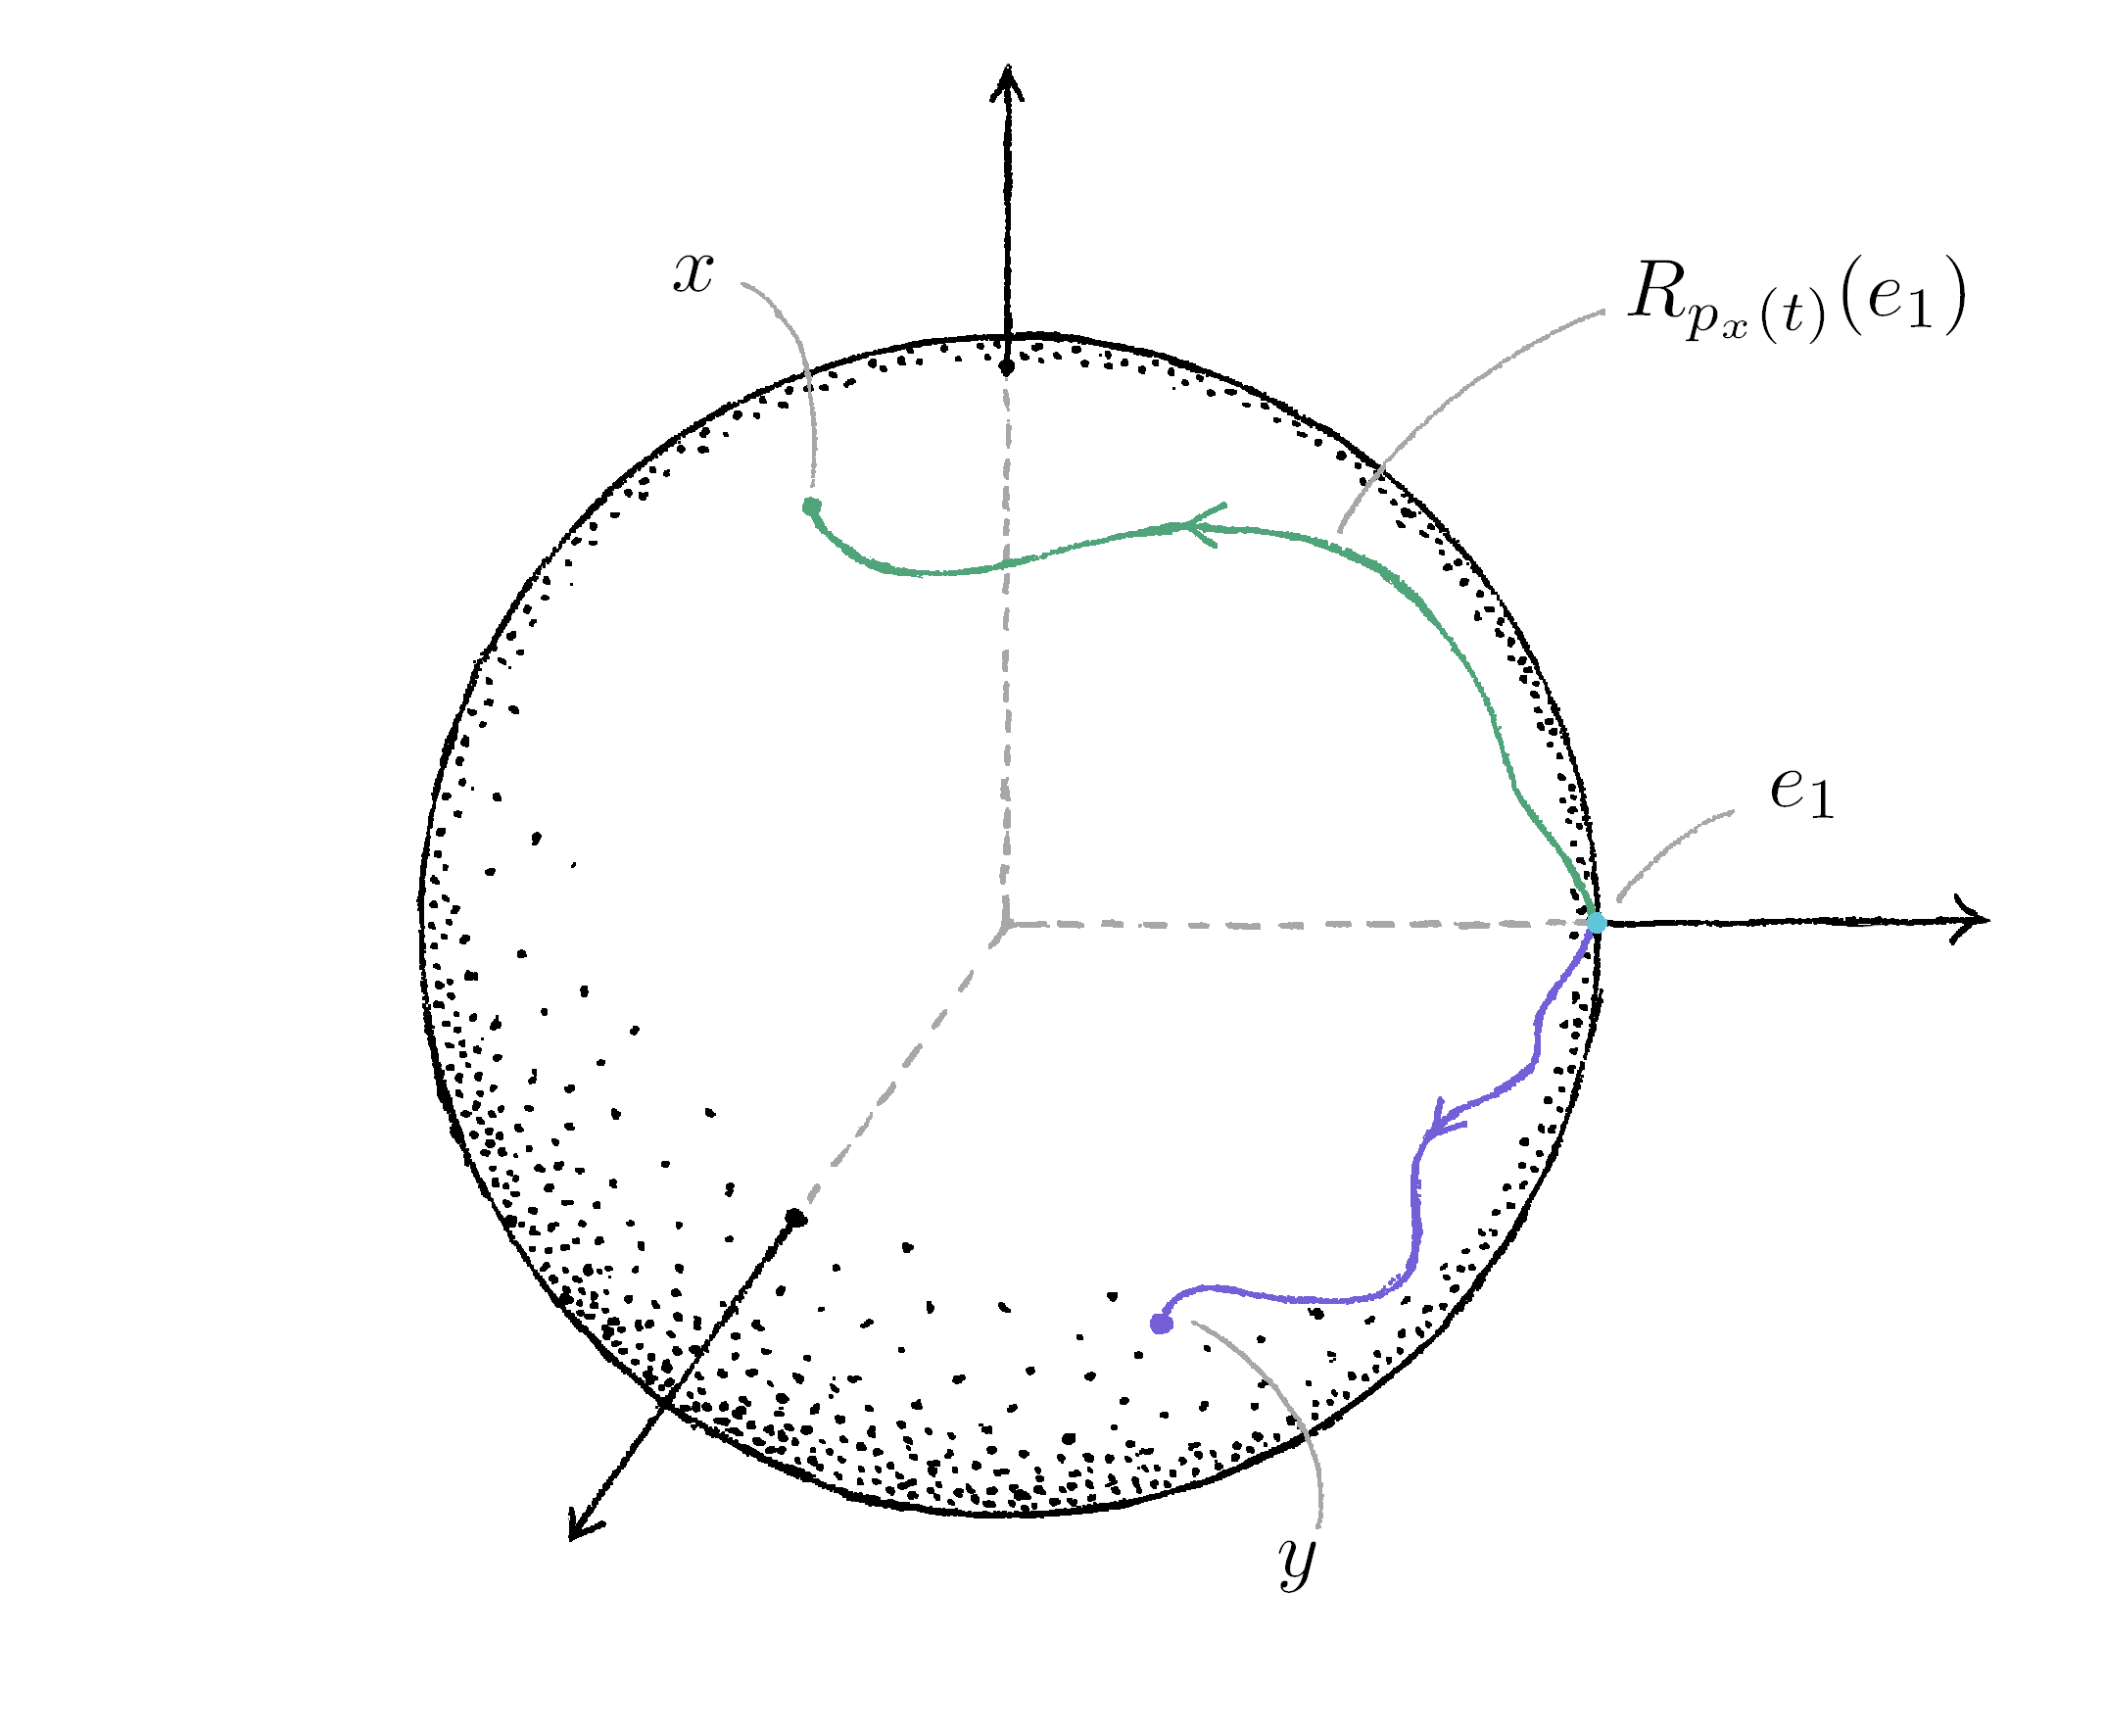
\includegraphics[scale=0.45]{figs/composing_paths/sphere_colour.png}
\caption{Here we depict the trajectories of $e_1$ in \sph{2} as it is evolved under paths in \gsok{3}, as decribed in \ref{transitive_action_on_sphere}, corresponding to points $x, y \in S^2$. Clearly, we can map $x$ to $y$ via $R_{p_x(1)}^{-1}\circ R_{p_y(1)}$.}
\label{compose_paths}
\end{figure}


For the second statement we proceed by induction. For $n = 2$ this is easy since
\[
\gsok{2} = \{\pmqty{\cos \theta & \sin \theta \\ -\sin \theta & \cos \theta}\mid \theta \in [0, 2\pi )\}.
\]
Clearly, for $x = (\cos\theta, \sin\theta) \in S^1$ we have a path
\[
p(t) = \pmqty{\cos (t\theta) & \sin (t\theta) \\ -\sin (t\theta) & \cos (t\theta)},
\]
such that $(1\ 0)p(t) = (\cos(t\theta)\ \sin(t\theta)$ which starts at $(1\ 0)$ and ends at $x$.
(insert figure of circle here)

Now assume the result is true for $n=k$ and consider \gsok{k+1} acting on $\rR^{k+1}$. We can write any $x \in S^k \subset \rR^{k+1}$ as $x = \cos\theta e_1 + \sin\theta y$ where $y \in \mbox{Span}\{e_2, \hdots, e_{k+1}\}$ is a unit vector. Choose a path $p_1(t)$ in \gsok{n} taking the form

\[
\begin{pmatrix}
  \begin{matrix}
  \cos(t\theta) & \sin(t\theta)  \\
  -\sin(t\theta) &   \cos(t\theta)
  \end{matrix}
  & \rvline & \bigzero
  \\
\hline

  \bigzero & \rvline &
  \ci{k-1}
\end{pmatrix}
\]
Observe that $R_{p_1(1)}(e_1) = \cos\theta e_1 + \sin\theta e_2$. Now, identify $\rR^k$ with $\mbox{Span}\{e_2, \hdots, e_{k+1}\}$. We know there exists a path $\bar{p}_2 : [0, 1] \to \gsok{k}$ such that $\bar{p}_2(0) = \mathcal{I}_k$ and $R_{\bar{p}_2(1)}(e_2) = y$ by the inductive hypothesis. By linearity $R_{\bar{p}_2(1)}(\sin(\theta) y) = \sin(\theta) y$. Now, we can define $p_2:[0, 1] \to \gsok{k+1}$ by
\[
p_2(t) =
\begin{pmatrix}
  1 & \rvline & 0
  \\
\hline

  0 & \rvline & \bar{p}_2(t)
\end{pmatrix}.
\]
Finally, define $p:[0, 1] \to \gsok{k+1}$ by
\[
p(t) =
\begin{cases}
p_1(2t)   & t \in  [0, \frac{1}{2}) \\
p_2(2t-1) & t \in  [\frac{1}{2}, 1].
\end{cases}
\]
By construction, $p(0) = \ci{k+1}$ and $R_{p(1)}(e_1) = \cos(\theta)e_1 + \sin(\theta)y = x$.
\end{proof}

\ul{Remark} Similar arguments apply to \gsuk{n} and \gspk{n} with very little change.

\begin{cor}
\gsok{n} is path-connected.
\end{cor}

\begin{proof}
For any $A \in \gsok{n}$ we construct a path from $A$ to \cin. By Lemma 1.2.5 the rows of $A$ form an orthonormal basis for $\rR^n$. Call these $r_1, \hdots , r_n$. By theorem 1.3.6 there exisits a path $p$ in \gsok{n} starting with \cin and ending with $p(1)$ which satisfies $R_{p_1(1)}(r_1) = e_1$. As matrices in \gsok{n} preserve orthonormality (by lemma 1.2.5) we see that $R_{p_1(1)}(r_i) \in \mbox{Span}\{e_2, \hdots , e_n\}$ for $i \geq 2$

Now let $s_2 = R_{p_1(1)}(r_2)$. By theorem 1.3.6, there exists a path $\bar{p}_2$ in \gsok{n-1} such that the corresponding path,
\[
p_2(t) =
\begin{pmatrix}
  1 & \rvline & 0
  \\
\hline

  0 & \rvline & \bar{p}_2(t)
\end{pmatrix},
\]
moves $s_2$ to $e_2$, ie $R_{p_2(1)}(s_2) = e_2$ (and $p_2(0) = \cin$). We can continue in this way to construct paths $p_i$ moving $r_i$ to $e_i$ but fixing $e_1, \hdots , e_{i-1}$. We can also compose these paths to obtain a path $p(t)$ such that $p(0) = \cin$ and $R_{p(1)}(r_i) = e_i$ for all $i$.

Finally, consider the $n\times n$ matrix obtained by stacking the images of $r_1, \hdots , r_n$ under $R_{p(t)}$:
\[
\begin{pmatrix}
  \horzbar & R_{p(t)}(r_1) & \horzbar \\
  \horzbar & R_{p(t)}(r_2) & \horzbar \\
  & \vdots &        \\
  \horzbar & R_{p(t)}(r_n) & \horzbar
\end{pmatrix}
\]
Notice that, for eact $t$, the rows are orthonormal, so this matrix is an element of \gsok{n} for all $t \in [0, 1]$. Moreover, at $t=0$ this matrix is
\[
\begin{pmatrix}
  \horzbar & r_1 & \horzbar \\
  \horzbar & r_2 & \horzbar \\
  & \vdots &        \\
  \horzbar & r_n & \horzbar
\end{pmatrix}
= A
\]
and at $t=1$
\[
\begin{pmatrix}
  \horzbar & e_1 & \horzbar \\
  \horzbar & e_2 & \horzbar \\
  & \vdots & \\
  \horzbar & e_n & \horzbar \\
\end{pmatrix}
= \cin
\]
Hence, we have constructe a path in \gsok{n} from $A$ to \cin.
\end{proof}

\section{Lecture 12 23/10/23}

Previously: 
\begin{itemize}
\item 1.3.6 \gson acts transitively on \sph{n-1}
\item 1.3.7 \gson is path-connected. 
\end{itemize}

\ul{Remark} Essentially the same arguments used in 1.3.6 \& 1.3.7 show

\begin{itemize}
\item \gsun, \gspn act transitively on \sph{2n-1} and \sph{4n-1} respectively.
\item \gsun , \gspn are path-connected. \gsln is also path connected, but the argument is different.
\end{itemize}

\begin{cor}
\gun is path connected by \gon has two path components (i.e. \ul{not} path connected).
\end{cor}

\begin{proof}
By 1.2.11, $\gun=\gsun \rtimes \guk{1}$. Topologically, $\gun \cong \gsun \times \sph{1}$ (forgetting the group structure), and is $\therefore$ path connected as \gsun and \sph{1} both are.

By 1.2.12, $\gon=\gson \rtimes \zZ_2$. Topologically this means $\gon \cong \gson \underset{\text{disjoint union}}{\amalg} \gson$. Hence $\gon$ has two path components, each $\cong \gson$. 
\end{proof}

\ul{Remark} $\zZ_2$ here corresponds to $\{I_n, \pmqty{\dmat{-1,1,\ddots,1}}\}$. The matrix $\pmqty{\dmat{-1,1,\ddots,1}}$ corresponds to a reflection in the hyperplane $\operatorname{span}\{e_2,\ldots,e_n\}$ (flipping the $e_1$ coordinate over). Notice that we can't have a continuous path from $I_n$ to $\pmqty{\dmat{-1,1,\ddots,1}}$ in $\gon$ as the determinant (which is continuous) would have to jump from $1$ to $-1$.

If we define a rotation of $\rR^n$ to be an origin fixing distance preserving map which can be linked via a continuous path of such maps to $I_n$, then we can deduce
\begin{itemize}
\item \gson is precisely the group of rotations of $\rR^n$,
\item \gon is precisely the group of rotations and reflections of $\rR^n$.
\end{itemize}

\ul{Final remark}:``Homogeneous spaces''.

If $G$ is a topological group and $H\subset G$ a subgroup, then the set of cosets $\quot{G}{H}$ ( or $_{H}\backslash ^{G}$) is a topological space with the quotient topology. $\quot{G}{H}$ is called a ``Homogeneous space'', as, when equipped with an appropriate geometry \quot{G}{H} ``looks'' the same at all points.

\ul{Examples} $\sph{n-1}\cong \quot{\gson}{\gsok{n-1}}\cong \quot{\gon}{\gok{n-1}}$, where \gsok{n-1} is identified with $\pmqty{\dmat{1,\gsok{n-1}}}\subset\gson$ etc.

$\sph{2n-1}\cong \quot{\gsun}{\gsuk{n-1}}\cong \quot{\gun}{\guk{n-1}}$

$\sph{4n-1}\cong \quot{\gspn}{\gspk{n-1}}$.

\subsection{Lie groups \& Lie Algebras}

\subsubsection{Manifolds}

Roughly speaking a manifold is a ``nice'' topological space such that a neighbourhood of each point ``looks like'' euclidean space of a fixed dimension. We can use the local euclidean property to transfer calculus (differential and with a bit more work integral) from $\rR^n$ to manifolds.

\begin{defn}
A topological $n$-manifold $M$ is a Hausdoff topological space with a countable basis for its topology, satisfying the following locally euclidean property: For any $x\in M$ there is an open set $x\in U\subset M$, and an open set $V\subset \rR^n$, and a homeomorphism $\phi:U \to V$.

(nice picture of torus, open sets, and arrow between it and $V$ in $\rR^n$).
\end{defn}

\ul{Remarks}
\begin{itemize}
\item[1)] $n$ is the ``dimension'' of the manifold.
\item[2)] The map $\phi$ is called a ``chart''.
\item[3)] A locally Euclidean space  which is a subset of some $\rR^m$ $m\geq n$ is automatically Hausdorff and has a countable basis for its topology.
\end{itemize}

\section{Lecture 13 25/10/23}

\ul{Previously} 2.1.1 A topological $n$-manifold $M$ is a Hausdoff topological space with a countable basis for its topology,which is locally euclidean, i.e. for each $x\in M  \exists U\subset M$ open with $x\in U$ and a homeomorphism $\phi:U \to V$, where $V\subset \rR^n$ is an open set. $\phi$ is a ``chart''. 

\begin{defn}
A family of charts $\{\phi_\alpha \mid \alpha \in \Lambda \}$ ($\Lambda$ an indexing set) on a manifold $M$ is called an \ul{atlas} if for each $x\in M$ $\exists \alpha \in \Lambda$ s.t. $x\in $ domain of $\phi_\alpha$.
\end{defn}

\ul{Remark} The inverse of any chart provides $M$ with a local coordinate system. See figure \ref{coord_patch}.

\begin{figure}
\center
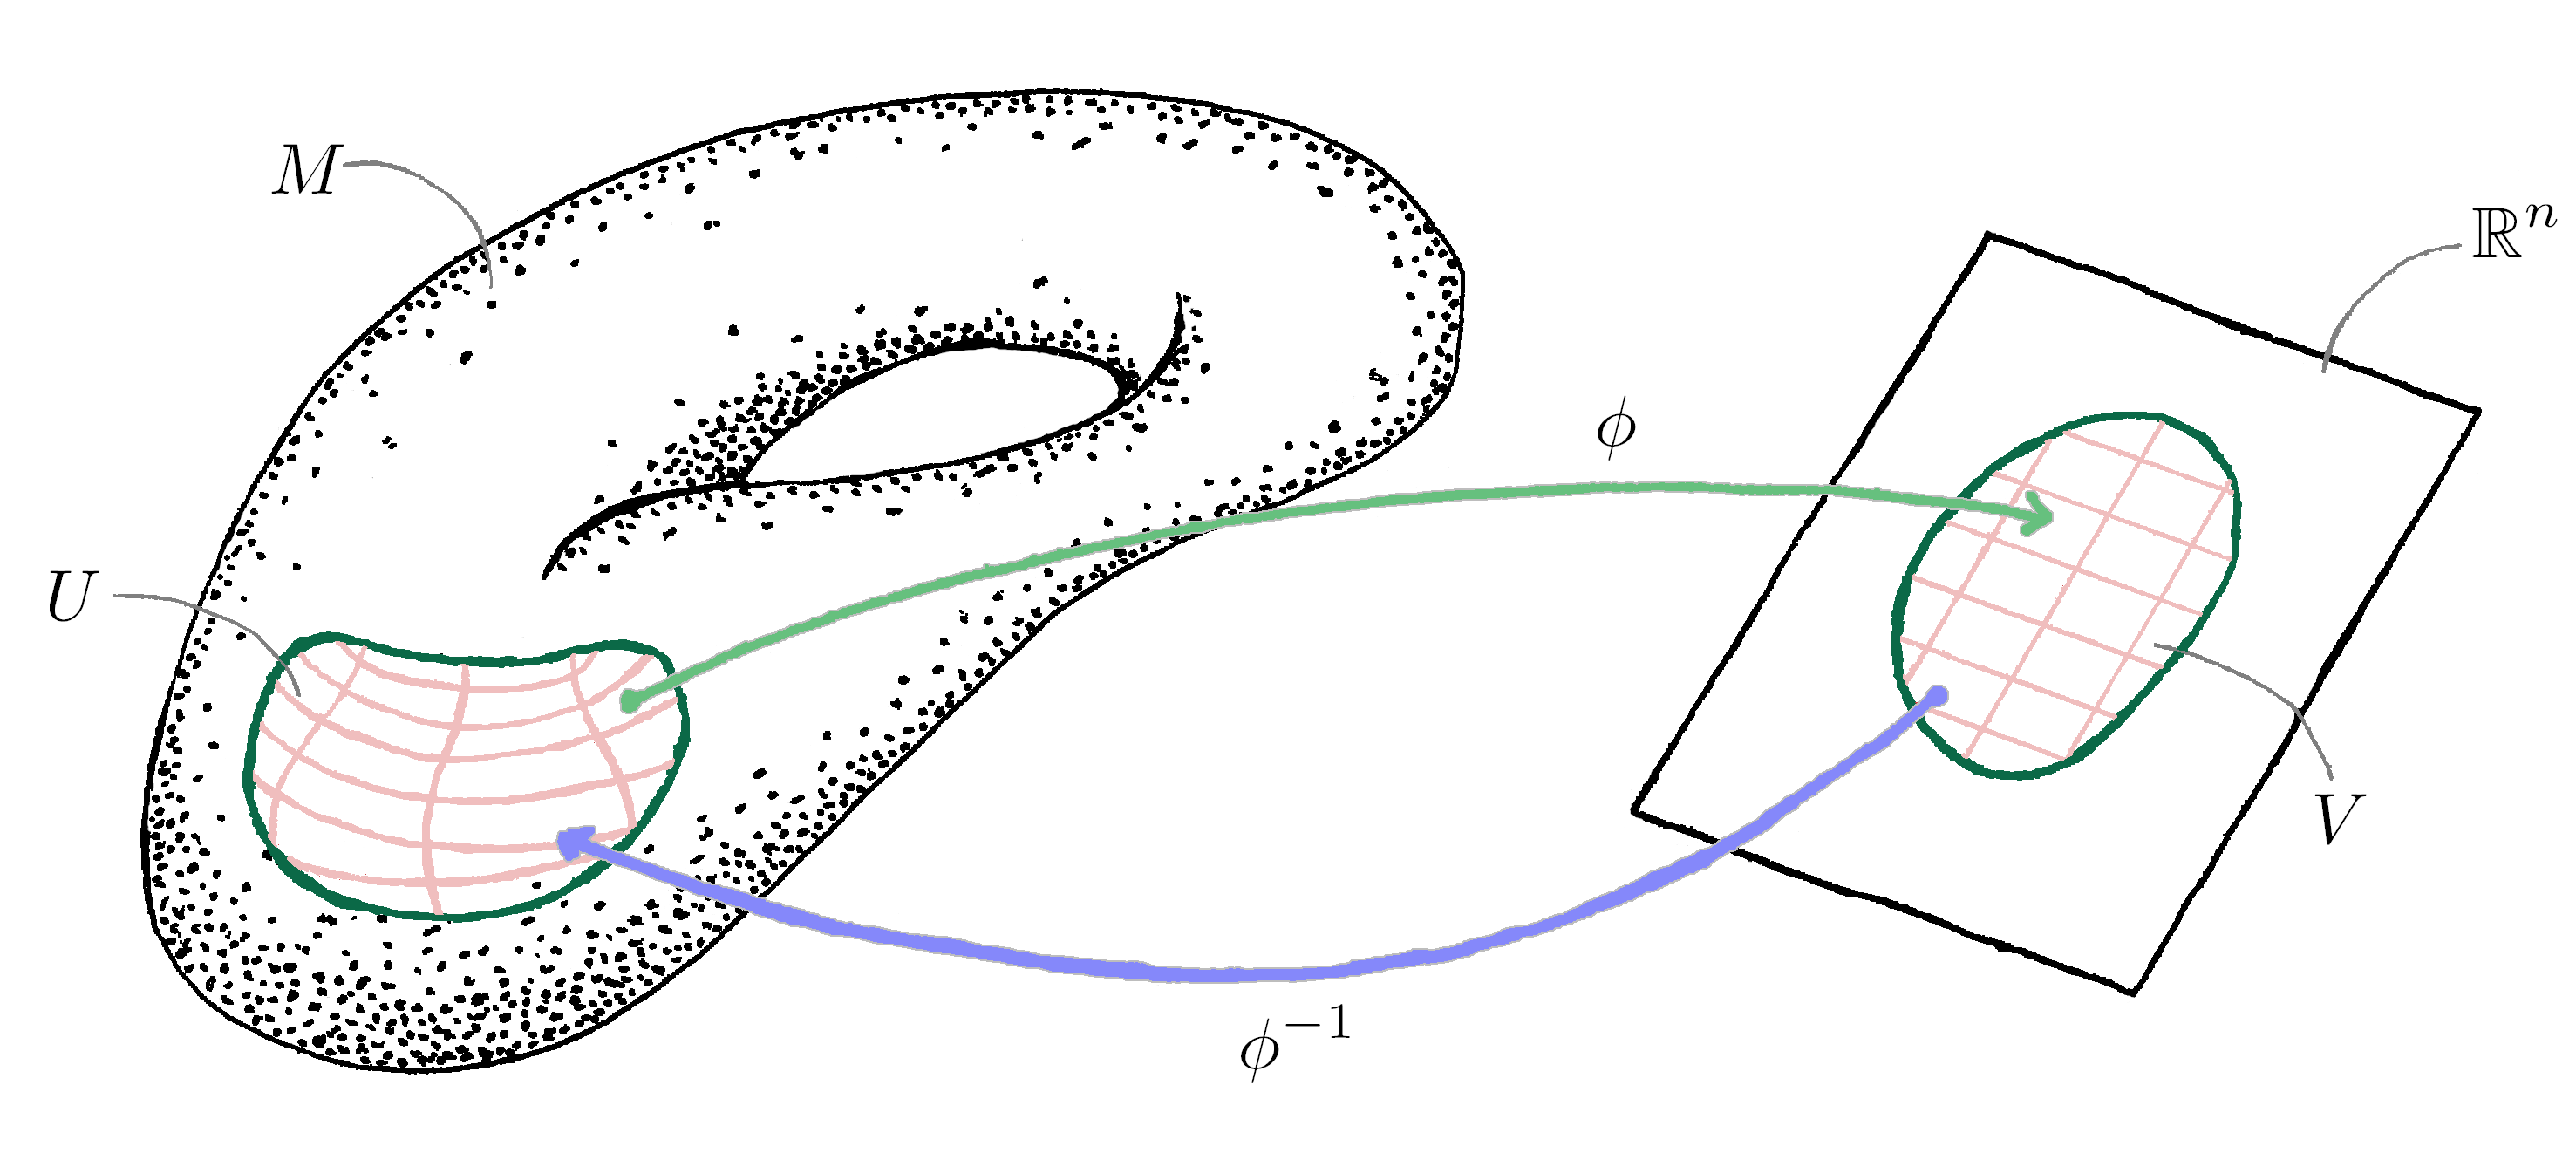
\includegraphics[scale=0.5]{figs/coord_patch/manifold_phi_inv.png}
\caption{The inverse of a chart $\phi$ provides $M$ with a local coordinate system. Coordinate lines in $V \subset \rR^n$ are mapped by $\phi^{-1}$ to continuous curves in $M$ which trace the local coordinate system on $M$.}
\label{coord_patch}
\end{figure}

(today upgrade definition of topological manifold to a smooth one)

We next describe what it means for a manifold to be \ul{smooth}. We use charts to interpret smoothness.

Given charts $\phi: U\to V$, $\theta: U' \to V'$ on $M$, assume $U\cap U' \neq \emptyset $. Then there $\exists h : \phi(U\cap U')\to \theta(U\cap U')$ such that the following diagram commutes

\begin{center}
\begin{tikzcd}[column sep=tiny]
& U\cap U' \ar[dl,"\phi \large|_{U\cap U'}"'] \ar[dr,"\theta \large|_{U\cap U'}"] & \\
\underset{\subset V \subset \rR^n}{\phi(U\cap U')}\ar[rr,"h"'] & & \underset{\subset V' \subset \rR^n}{\theta(U\cap U')}
\end{tikzcd}
\end{center}

$h:=\theta \large|_{U\cap U'}\circ \phi \large|_{U\cap U'}^{-1}$. Observe that $h$ is a homeomorphism between open sets in $\rR^n$. As a map of Euclidean spaces, it makes sense to ask: is $h$ smooth, i.e. infinitely differentiable? $h$ is called a ``transition function''.

\begin{defn}
An atlas $\{\phi_\alpha\}$ is said to be a \ul{smooth atlas} if all transition functions are smooth $(\cinf)$ with smooth inverses.
\end{defn}

(note smooth functions like $x^3$ don't necessarily have smooth inverses everywhere).

Two overlapping charts are said to be ``smoothly compatible'' if the corresponding transition function is smooth. 

Given a smooth atlas, we could expand the atlas by including all possible charts which are smoothly compatible with each other. So any smooth atlas can be expanded to a ``maximal $\cinf$ atlas''.

\begin{defn}
A smooth manifold is a topological manifold equipped with a maximal smooth atlas. Such a maximal atlas is called a ``\cinf structure''
\end{defn}

(question about uniqueness of maximal atlases - 28 different ones for \sph{7}, Milnor came up with an example. Exotic differentiable structures)
 
\ul{Remark} One of the benefits of a smooth structure is that it allows us to define an ambiguous  way whether `objects' defined on the manifold (e.g. functions) are smooth or not.

\ul{Examples} 
\begin{itemize}
\item Dim 0: one-point spaces (or disjoint unions of one point spaces). $\sph{0}=\{1,-1\}$. 
\item Dim 1: \rR or \sph{1}. (other manifolds with boundary but not defining that).
\item \ul{Dim 2} (theorem) Two families
\begin{itemize}
\item the ``orientable'' family, \sph{2}, $\tor{2}=\sph{1}\times \sph{1}$, $\tor{2}\underset{\text{connected sum}}{\#}\tor{2}$,  $\tor{2}\#\tor{2}\# \tor{2}$, $\ldots$ (connected sum is removing a disk from each and joining with a cylinder).
\item the ``non-orientable'' family: $\underbrace{\rpk{2} (\text{real projective space}), K (\text{Klein bottle})}_{\text{these don't live in }\rR^3}$, $\sph{2}$ with $n$ discs removed with $n$ mobius bands glued in.
\end{itemize}
\item In any dimension $\rR^n$ is a manifold with atlas consisting of a single chart $\{\mathrm{id}_{\rR^n}\}$. Ditto $\mnf (\cong \fF^{n^2})$. 
\item We also have an $n$-sphere $\sph{n}\subset \rR^{n+1}$. $\sph{n}=\{(x_1,\ldots,x_{n+1})\mid \sum\limits_{i=1}^{n+1}x_i^2=1\}$.
\end{itemize}

\section{Lecture 14 27/10/23}

To see that \sph{n} is a manifold we describe an atlas involving $2n+2$ charts. Take open hemispheres about the points $\pm e_1, \pm e_2, \ldots,\pm e_{n+1}$. We define a chart for each of these half spheres to $\rR^n = $ space orthogonal to $\pm e_i$ by projection (picture of projection). This is a smooth atlas as the transition functions, which are compositions of projections are clearly smooth maps. (There's also an atlas with just two charts, using stereographic projection from the poles. Messy exercise).

\ul{Exercise} If $M$ and $N$ are manifolds, show that $M\times N$ (with the product topology) is a also a manifold with dimension $\dim M +\dim N$.

\ul{Example} 2-torus $\tor{2}=\sph{1}\times \sph{1}$. 3-torus $\tor{3}=\sph{1}\times \sph{1}\times \sph{1}$, $n$-torus $\tor{n}=\sph{1}\times \ldots \times \sph{1}$. Tori are extremely important in the theory of Lie groups.  (they're abelian groups).

\begin{defn}
If $M^m$ (notation for dimension of a manifold) is a $\cinf$- manifold and $N\subset M$ is a subset equipped with the subspace topology (intersect open sets with subset) then $N$ is a dimension $n(<=m)$ \ul{submanifold} if for every $x\in N$ there is a chart $\phi:U\to V$ \ul{of M} with $x\in U$, such that $\phi(U\cap N)=\phi(U)\cap \left(\underset{\subset \rR^m=\rR^n \times\rR^{m-n}}{\rR^n\times \{0\}}\right)$. The restriction of charts taking this form to $N$ gives an atlas for $N$.
\end{defn}

\ul{Examples} \begin{itemize}
\item[i)] \sph{n} is a submanifold of $\rR^{n+1}$. 
\item [ii)] The equator $\sph{n-1}\subset \sph{n}$ is a submanifold of $\sph{n}$.
\item[iii)] $\sph{1}\times \{p\}\subset \sph{1}\times\sph{1}=\tor{2}$ is a circular submanifold of \tor{2}.
\end{itemize}

\ul{Remark} There are ways of detecting submanifolds which are easier than finding atlases.
 
\begin{thm}
(Whitney embedding theorem) Any smooth $n$-manifold can be $\underset{\text{(diffeomorphic)}}{\text{realised}}$ as a submanifold of $\rR^{2n}$. (No proof included)
\end{thm} 

\ul{Maps between manifolds}

\begin{defn}
A map of smooth manifolds $f:M\to N$ is \ul{smooth} if for every $x\in M$ and every chart $\theta:U'\to V'$ of $N$ with $f(x)\in U'$ and every chart $\phi:U\to V$ for $M$ with $x\in U$ and $f(U)\subset U'$, there is a \ul{smooth} map $\bar{f}$ making the following square commute:
\end{defn}

\begin{center}
\begin{tikzcd}
  U\subset M \arrow{d}{\phi} \arrow{r}{f\big|_U}
    & f(U)\subset N \arrow{d}{\theta\big|_{f(U)}} \\
  V \arrow{r}{\bar{f}}
&\theta(f(U)) \end{tikzcd}
\end{center}

\ul{Idea} $\bar{f}$ is the 'same' as $f$ just viewed through charts. Need to use charts here as smooth only makes sense in Euclidean spaces. 

\begin{defn}
A bijection of smooth manifolds $f:M\to N$ is a \ul{diffeomorphism} if it is smooth with smooth inverse.
\end{defn}

\begin{defn}
A \ul{Lie group} is a group $G$ which is also a smooth manifold for which the multiplication map $G\times G\to G$ and the inverse map $G\to G$ are both smooth.
\end{defn}
 
(Aside: Gromoll Meyer sphere $_{\gspk{1}}\slash ^{\gspk{2}} \backslash _{\gspk{1}}$ biquotient. Exotic sphere with non-negative curved)
 
\section{Lecture 15 06/11/23}

\ul{Previously}

\begin{itemize}
\item Manifold $M^n$ is a topological space locally $\cong \rR^n$. Charts give a way of doing calculus locally on a manifold. Transition functions from a smooth atlas give us a way of making the local calculus global: they guarantee that calculus in one chart agrees with that in any overlapping chart.
\item Smooth functions $f:M \to N$ are those which are smooth when viewed through charts.

\begin{center}
\begin{tikzcd}
  U\subset M \arrow{d}{\phi} \arrow{r}{f\big|_U}
    & f(U)\subset N \arrow{d}{\theta\big|_{f(U)}} \\
 V \arrow{r}{\bar{f}}
&W \end{tikzcd}
\end{center}
i.e. want $\bar{f}$ to be smooth for any suitable choice of charts in $M,N$.
\item Lie groups: this is a group $G$ which is also a $\cinf$ manifold s.t. multiplication $G\times G\to G$ \& inverse $G\to G$ are both \cinf.
\end{itemize} 

Consider a differentiable map $g:\rR^n\to \rR^m$. The derivative of $g$ is described by the Jacobian  matrix. Writing $g=(g_1,g_2,\ldots, g_m)$,

\[\pmqty{\pdv{g_1}{x_1} & \ldots & \pdv{g_1}{x_n}\\ 
\vdots & \ldots & \vdots \\ 
\pdv{g_m}{x_1} & \ldots & \pdv{g_m}{x_n} }\]

At some point $p\in \rR^n$ the Jacobian has "a rank" = max no of linearly independent rows/columns. (A result of linear algebra says that the row and column rank are the same.) For a differentiable map $f:M\to N$ the rank of $f$ at $p\in M$ is the rank of the Jacobian matrix $\bar{f}$ at the point corresponding to $p$ in $\rR^n$. 
\ul{NB} This concept of rank for maps between manifolds is well defined, i.e. is independent of the charts used to define $\bar{f}$. This is a consequence of the smooth atlas definition (smooth transition functions).

\begin{defn}
$f:M^m\to N^n$ a \cinf map, $m\geq n$.
\begin{itemize}
\item[a)] A point $p\in M$ at which (less than maximal) $\rank_{p}{f}<n$ is called a \ul{critical value} of $f$, and $f(p)$ is a \ul{critical value}.
\item[b)] A point $y\in N$ is a \ul{regular value} of $f$ if $\rank_{p}{f}=n$ (i.e. maximal) $\forall p \in f^{-1}(\{y\})$ (preimage of $y$).
\end{itemize}
\ul{Important convention}
Every point of $N$ which is \ul{not} in image of $f$ is declared to be regular.
\end{defn}

\begin{thm}
(The implicit Function Theorem - manifolds version).

If $y\in N$ is a regular value of $f:M^m\to N^n$ ($m\geq n$) a smooth map, then the pre-image $f^{-1}(\{y\})$ is a smooth submanifold of $M$ with dimension $m-n$. 

(No proof)
\end{thm}
 
This is particularly useful when $M=\rR^n$ or $M=\mnf (\cong \fF^{n^2})$.

e.g.

$f:\rR^n \to \rR$ defined by $f(x_1,x_2,\ldots, x_n)=\sum\limits_{i=1}^n x_i^2$. Then $f^{-1}(\{1\})=\sph{n-1}$. We conclude from IFT (2.1.11) that $\sph{n-1}$ is a manifold of dimension $n-1$ provided that $1$ is a regular value of $f$.  $\jac{f}=(\pdv{f}{x_1},\pdv{f}{x_2},\ldots,\pdv{f}{x_n})$ $=(2x_1,2x_2,\ldots,2x_n)$. This has rank $1$ unless $(2x_1,2x_2,\ldots,2x_n)=0$, but $0\not\in f^{-1}(\{1\})$, so this does not occur. So $1$ \ul{is} a regular value of $f$.

\ul{Applications to groups of matrices}

Firstly, since $\mnr\cong \rR^{n^2}$ and $\rR^{n^2}$ is trivially a manifold, $M_n(\rR^n)$ is a manifold. Next, observe that any open subset of a manifold is again a manifold under restriction of the topology and charts.

$\glnr = \{A\in \mnr \mid \det A\neq 0\}$. This is an open subset of $\mnr$ ($\glnr = \det ^{-1}(\rR \setminus \{0\})$. (preimage of an open set under a continuous function is open, $\rR \setminus \{0\}$ is open). $\therefore \glnr$ is a manifold of dim $n^2$. (Similar comments for \glnc and \glnh).

\section{Lecture 16 08/11/23}

Last time:

\begin{itemize}
\item \glnr is a manifold of dimension $n^2$. (because it's an open subset of $\mnr\cong \rR^{n^2}$. Similar comments for \glnc, \glnh .
\item Differentiable map $f:M^n\to N^n$, with $m\geq n$, then the rank of $f$ at $p\in M$ $\underset{\text{defn}}{=}$ rank of Jacobian map of $\bar{f}$ ($f$ viewed through chart, i.e. as a map between open subsets $\rR^m$, resp. $\rR^n$.
\item $y\in N$ is a regular value of $\rank_p f = n$ (maximal!) $\forall p \in f^{-1}(\{y\})$.
\item Implicit function theorem: if $y$ is a regular point, then pre-image $f^{-1}(\{y\})$ is a smooth submanifold of $M$ with dimension $m-n$.
\end{itemize}

\ul{Examples of Lie Groups}
\begin{itemize}
\item[(i)] $\gsln = \{A\in \mnr \mid \det A=1\}$. Consider $\det:\glnr\to \rR$. So $\gsln = \det^{-1}(\{1\})$.  By the IFT we will see that \gsln is a submanifold of \glnr with dimension $n^2-1$ and hence a Lie group since the multiplication and inversion in \gsln are the restrictions of the smooth multiplication and inversion in \glnr. We $\therefore$ need  to show that $1\in \rR$ is a regular value for $\det$, i.e. we need to show that the rank of $\det \neq 0$ at each $A\in \glnr$ with $\det A = 1$, i.e. the derivative at $A$ (in some direction through \glnr is non-zero). Consider the path $p(t)=(1-t)A$. $\det p(t) = (1-t)^n \det A = (1-t)^n$. $p(t)\in \glnr$ for $t$ small. Differentiating $\dv{t} \det \eval{p(t)}_{t=0}=\dv{t}\eval{(1-t)^n}_{t=0}=\eval{n(1-t)^{n-1}}_{t=0}=n\neq 0$.
Thus the rank of the $\det$ is maximal (i.e.$=1$), at every $A\in\gsln$ as required.
\item[(ii)] $\gson=\{A\in\mnr \mid AA^T=I_n\}$. Observe that $AA^T$ is symmetric, i.e. $(AA^T)^T=AA^T$. Let $S_n(\rR)=\{A\in \mnr \mid A \text{ is symmetric i.e. } A^T=A\}$. Notice that $S_n(\rR)\cong \rR^{\frac{1}{2}n(n+1)}$ as any element of $S_n(\rR)$ is determined by its upper/lower triangle of entries. So $S_n(\rR)$ is a manifold! 

Define $f:\underset{\cong \rR^{n^2}}{\mnr} \to \underset{\cong \rR^{\frac{1}{2}n(n+1)}}{S_n(\rR)}$, by $f(A)=AA^T$. ($f ``=" \bar{f}$)) Apply IFT to $f$. 

\ul{Claim} every element of $S_n(\rR)$ in $f^{-1}(\{I_n\})$ is a regular value of $f$. Choose $A,B \in \mnr$ and consider the path $A+tB\in \mnr$. Differentiating $f$ along this path at $t=0$: $df_A(B)$ (Deriv of $f$ at $A$ (i.e. $t=0$) in direction of $B$).
\begin{align*}
df_A(B)&=\dv{t}\eval{f(A+tB)}_{t=0}\\
&=\lim_{t=0} \frac{f(A+tB)-f(A)}{t}\\
&=BA^T+AB^T
\end{align*}
Calculation: exercise. Notice that $BA^T+AB^T$ is also symmetric! Thus $df_A:\mnr\to S_n(\rR)$. The claim follows if we can show $df_A$ is surjective (since $df_A$ is linear) for each $A\in f^{-1}(I_n)$. To see this: for any $C\in S_n(\rR) $ we can easily check that by setting $B=\frac{1}{2}CA$, we obtain $df_A(B)=C$. $\therefore$ by IFT $\gson =f^{-1}(\{I_n\})$ is a manifold of dimension $n^2-\frac{1}{2}n^2-\frac{1}{2}n=\frac{1}{2}n(n-1)$.

\end{itemize}

\section{Lecture 17 10/11/23}
Last time:

Showed \gson is a submanifold of \mnr of dimension $\frac{1}{2}n(n-1)$ using Implicit Function Theorem.

To show that \gson is a Lie group we simply observe that the multiplication and inverse operations agree with those (where defined) in \mnr, and hence are smooth.

\subsubsection{Tangent Spaces}

Consider a submanifold $M^m\subset \rR^n$. Let $p\in M$ and consider a smooth path $\gamma:(-\epsilon,\epsilon)\to M\subset\rR^n$ with $\gamma(0)=p$. (small picture of gamma in manifold, with velocity vector).

The velocity vector $\gamma'(0)$ is  a vector in $\rR^n$. Now consider the set of \ul{all} such paths $\gamma$. From this we get a set of velocity vectors $\subset \rR^n$. Intuitively it is clear that this set is an affine vector space, i.e. a vector space translated to the point $p$.

\begin{defn}
\begin{itemize}
\item[(a)] The \ul{tangent space} to $M\subset\rR^n$ to $p$, \tpm , is the set of velocity vectors to $M$ at $p$.
\end{itemize}
\end{defn}

\ul{Aim}: formulate an intrinsic notion of tangent space, i.e. not depending on a choice of embedding into some $\rR^n$.

\ul{Observation}: Given a path $\gamma$ through $p$ in $M$ \ul{as before}, and a differentiable function $f:M\to \rR$, consider the composition $f\circ \gamma:(-\epsilon,\epsilon)\to \rR$. This is differentiable. We can think of this derivative as a directional derivative of $f$ in the direction of $\gamma'(0)$. We can therefore identify velocity vectors $\gamma'(0)$ at $p$ with directional derivative operations, i.e. with differential operators. The point is that this makes as much sense for abstract manifolds as for submanifolds of $\rR^n$.

Denote the set of all \cinf real-valued functions on $M$ by  \cinfm. 

\begin{defn}
Given a smooth curve $\gamma(t)$ on $M$ with $\gamma(0)=p$, the \ul{tangent vector} to $\gamma$ at $p$ is a map $\gamma'(0):\cinfm \to \rR$ given by $\gamma'(0)(f)=\dv{t}\eval{f\circ \gamma(t)}_{t=0}$.
\end{defn}

Given a chart $\phi:\underset{\subset M}{U}\to \underset{\subset \rR^m}{V}$, we can use the standard coordinates $(x_1,x_2,\ldots, x_m)$ in $V$, $x_i :V\to \rR$, to obtain a local coordinate system in $M$, given by $(x_1\circ \phi, \ldots, x_m\circ \phi)$. For simplicity, we'll call these coordinates on $M$, $(x_1,\ldots, x_m)$.

Assume that $p\in U$ and $\phi(p)=0\in V\subset \rR^m$. In these coordinates we have $\gamma(t)=(\gamma_1(t),\ldots,\gamma_m(t))$, ($\gamma_i :(-\epsilon,\epsilon)\to \rR$) and $\therefore$

\begin{align*}
\dv{t}\eval{f\circ \gamma(t)}_{t=0}&=\dv{t}\eval{f(\gamma_1(t),\ldots,\gamma_m(t))}_{t=0}\\
&\underset{\text{chain rule}}{=}\sum_{i=1}^{m} \pdv{f}{x_i}(p)\gamma_i'(0)\\
&=\left(\sum_{i=1}^{m} \gamma_i'(0)\pdv{x_i}(p)\right) (f)
\end{align*}

where $\pdv{x_i}(p)$ is the tangent vector to the $x_i$ coordinate line at $p$, i.e. $(0,\ldots,0,\underset{i^{th} \text{ place}}{t},0,\ldots,0)$ in coords of U.

$\therefore \gamma'(0) = \sum_{i=1}^{m} \gamma_i'(0)\pdv{x_i}(p)$ $(*)$.

Observe that this only depends on the derivative of $\gamma$ at $p$.

\addtocounter{thm}{-2}
\begin{defn}
\begin{itemize}
\item[(b)] The \ul{tangent space} \tpm for any manifold $M$ is the set of velocity vectors (as defined above) to $M$ at $p$. The following is evident from $(*)$.
\end{itemize}
\end{defn}

\addtocounter{thm}{1}

\begin{lemma}
\tpm is a vector space of dimension $=\dim M$, and given local coordinates system $(x_1,x_2,\ldots, x_m)$ around $p$, a basis for \tpm is given by 
\[\{\pdv{x_1}(p),\ldots, \pdv{x_m}(p) \}\]
\end{lemma}

Notice that \tpm is independent of local coord systems, since tangent vectors themselves are indep. of local coords.

\section{Lecture 18 13/11/23}

Last time:

\begin{itemize}
\item tangent vector to a manifold $M$ at $p\in M$ is a directional differentiation operator at $p$. (Acting on smooth functions $M\to \rR$).
\item Tangent space \tpm is the set of all tangent vectors at $p$.
\item $\tpm = \operatorname{span}\{\pdv{x_1}(p),\ldots, \pdv{x_n}(p) \}$, where $(x_1,x_2,\ldots, x_n)$ is any local coordinate system on $M$ about $p$, and $\pdv{x_i}$ are the usual partial differentiation operations.
\end{itemize}

The collection of all tangent spaces $\bigcup\limits_{p\in M} \tpm^n$ has the structure of a manifold (non-compact!) of dimension $2n$. This is denoted $\tm$ and is called the "tangent bundle".

\ul{Examples}
\begin{itemize}
\item[(i)] $\tqn{p}{\rR^n}\cong \rR^n$. Consider a path $\gamma(t)=p+vt$ for some $v\in \rR^n$, $\gamma'(0)=v$. Thus the corresponding tangent (velocity) vector is $v$. 

Alternatively natively consider $\dv{t}\eval{f(p+vt)}_{t=0}$. If $v=\sum \lambda_i e_i$ then this is 
\begin{align*}
&sum \pdv{f}{x_i}\lambda_i \quad \text{by the chain rule.}\\
&=\left(\sum \lambda_i \pdv{x_i}\right)(f)
\end{align*}
So $\sum \lambda_i \pdv{x_i}$ is the tangent vector corresp to $v=\sum \lambda_i e_i$. The correspondence $\tqn{p}{\rR^n}\cong \rR^n$ is precisely $\sum \lambda_i \pdv{x_i} \leftrightarrow \sum \lambda_i e_i$.

\item[(ii)] $\tqn{A}{\mnr} \cong \mnr$. (Essentially a special case of (i)). Consider a path $\gamma(t)=A+tB$ for some $B\in \mnr$. Clearly $\gamma'(0)=B$. Alternatively, consider $\dv{t}\eval{f(A+tB)}_{t=0}$. Let $v_{ij}:\mnr \to \rR$ be the function which picks out the $(i,j)^{th}$ entry. Standard coordinates on \mnr.
\begin{align*}
\dv{t}f(A+tB)&\underset{\text{chain rule}}{=}\sum_{i,j} \pdv{f}{v_{ij}}b_{ij}\\
&=\left(\sum_{i,j}\pdv{f}{v_{ij}}b_{ij}\right)(f)
\end{align*}
So $\sum_{i,j}\pdv{f}{v_{ij}}b_{ij}$ is our tangent vector which we can identify with matrix $(b_{ij})=B$.

\item[(iii)]  $S_n(\rR)=\{(\nn) \text{ symmetric matrices }\}\cong \rR^{\frac{1}{2}n(n+1)}$. Same argument as in (ii) shows that $\tqn{A}{S_n(\rR)}\cong \S_n(\rR)$
\item[(iv)]  $\tqn{A}{\glnr}\cong \mnr$. We can see this two ways:
\begin{itemize}
\item[(a)] Since \glnr is an open subset of \mnr
\item[(b)] using same argument as (ii) after noting that for $A\in \glnr, B\in \mnr$, the path $A+tB$ lies in \glnr for $t close to 0$.
\end{itemize}
\end{itemize}

\begin{defn}
Given a differentiable map $f:M^n\to N^n$, the derivative of $f$ at $p\in M$, $\dfp$ is a map $\dfp:\tpm\to\tqn{f(p)}{N}$ given by $\dfp(X)=X(g\circ f) \forall g\in \cinfn{N}, \forall X\in \tpm$.
\end{defn}

\ul{Idea} Given a differentiable path $\gamma(t)$ through $p\in M$, $f(\gamma(t))$ is a differentiable path through $f(p)$ in $N$. If $X\in\tpm$ is the tangent vector $\gamma'(0)$ then $\dfp(X)$ is the tangent vector corresp. to $f(\gamma(t))$ at $f(p)$. (picture of path and image of path, tangent vectors etc)

\begin{lemma}
\dfp is a linear map.
\end{lemma} 
\begin{proof}
Trivial, from definition of \dfp.
\end{proof}

The individual derivatives \dfp can be assembled into a 'total' derivative $\df:\tm\to\tn{N}$ between tangent bundles.

\ul{Remarks}
\begin{enumerate}
\item Given coordinate systems about $p$ and $f(p)$ we obtain bases for \tpm and \tqn{f(p)}{N} and with respect to these bases, \dfp is given by a matrix. This is just the usual Jacobian matrix.
\item We can now re-interpret the notions of regular/critical points in terms of \dfp being surjective/ not surjective.
\item Previously we saw a map $f:\mnr \to S_n(\rR)$, $f(A)=AA^T$ we decided that \dfq{A} is a map $\mnr \to S_n(\rR)$. In reality $\dfq{A}:\underset{\cong\mnr}{\tqn{A}{\mnr}}\to \underset{\cong S_n(\rR)}{\tqn{AA^T}{S_n(\rR)}}$
\end{enumerate}

\ul{Vector Fields}
\begin{defn}
A (tangent) vector field on a smooth manifold $M$ is a choice of tangent vector at each $p\in M$, i.e. a rule which assigns $X(p)\in\tpm$ to each $p\in M$.
\end{defn}

Given a coord system $\xonen$ locally on $U\subset M$. We can express (locally) a vector field on $U$ as $\sum \lambda_i(p)\pdv{x_i}(p)$. Here $\lambda_i:U\to \rR$. We say the vector field is \ul{smooth} if the $\lambda_i$ are all smooth. The vector field is globally smooth (which we will assume from now on) if it is smooth in every chart. This is a well-defined concept, as the notion of smoothness is the same viewed from any charts in a smooth atlas.

\section{Lecture 19 15/11/23}

Last time:

\begin{itemize}
\item A tangent vector field on manifold $M$ is a choice of tangent vector in \tpm for each $p \in M$. This choice is assumed to be smoothly varying with $p$.
\end{itemize}

From now on we will use the term vector field to mean tangent vector field.

\ul{Remark}: A flow on $M$ is a one-parameter, smoothly varying, family of diffeomorphisms $M \to M$. (for example, flow of air around the earth) (TODO: insert figure of flow here). Differentiating a flow gives a vector field. Conversely,  vector field can be integrated to give a flow.

\subsubsection{Lie Algebras}

Let $X, Y$ be vector fields on $M$.

\begin{defn}
The Lie bracket of $X$ and $Y$, denoted $[X, Y]$ is\footnote{multiplication on the R.H.S. makes sense if vector fields are interpreted as differential operators.}
\[ [X, Y] = XY - YX. \]
\end{defn}

\begin{lemma}
$[X, Y]$ is a vector field on $M$. (ie it is a first order differential operator, not second order)
\end{lemma} 

\begin{proof}
Let $f \in \cinfn{M}$. So $XY(f) = X(Yf)$ etc. Note, $Yf \in \cinfn{M}$. With respect to a local coordinate system $(x_1,x_2,\ldots, x_n)$ we have
\[ X = \sum_i \lambda_i \pdv{x_i}, \quad Y = \sum_i \mu_i \pdv{x_i}, \]
for some $\lambda_i , \mu_i \in \cinfn{M}$.

Computing, we have
\begin{align*}
XYf - YXf &=  \sum_{i,j} \left(\lambda_i \pdv{\mu_j}{x_i} \pdv{f}{x_j} 
                       - \mu_j \pdv{\lambda_i}{x_j} \pdv{f}{x_i}\right) \\
          &+ \sum_{i,j} \lambda_j\mu_j\left( \pdv{^2f}{x_i\partial x_j}
           - \pdv{^2f}{x_j\partial x_i} \right).
\end{align*}
But the second partial derivatives commute.
\[ \therefore [X, Y](f) = \sum_{i,j} \left(\lambda_i \pdv{\mu_j}{x_i} \pdv{f}{x_j} 
                       - \mu_j \pdv{\lambda_i}{x_j} \pdv{f}{x_i}\right). \]
\[ \therefore [X, Y] = \sum_{i,j} \left(\lambda_i \pdv{\mu_j}{x_i} \pdv{x_j} 
                       - \mu_j \pdv{\lambda_i}{x_j} \pdv{x_i}\right). \]
\end{proof}

\ul{Remark}: This has a nice interpretation in terms of flows and is sometimes called a Lie derivative. One can define a way to push/pull $Y$ along the flow of $X$ and differentiate it, this gives a notion of differentiating $Y$ with respect to $X$. We won't explore this further here.

\begin{lemma}
The Lie bracket has the following properties:
\begin{enumerate}
\item It is bilinear.
\item It is anti-symmetric (ie $[X, Y] = - [Y, X]$).
\item It satisfies the "Jacobi identity":
\[ [[X, Y], Z] + [[Z, X], Y] + [[Y, Z], X] = 0. \]
\end{enumerate}
\end{lemma}

\begin{proof}
Properties 1 and 2 are trivial. For 3 we can simple write out each term and add. ie
$[[X, Y], Z] = [XY - YX, Z] = XYZ - YXZ - ZXY + ZYX$ etc. (exercise!)
\end{proof}

We now focus on vector fields on Lie groups.

For $g \in G$ ($G$ a Lie group) we have diffeomorphisms $L_g:G\to G$ given by $L_g(h) = gh$ (ie by left multiplication) and $R_g:G\to G$ given by $R_g(h) = hg$. We will concentrate on $L_g$ but everything will hold true for $R_g$ also. We have $dL_g : T_hG \to T_{gh}G$ for any $h \in G$.

\begin{defn}
A vector field $X$ on $G$ is left-invariant if $dL_g(X) = X \,\, \forall g \in G$. ie $dL_g(X_h) = X_{gh} \,\, \forall g, h \in G.$
\end{defn}
A similar definition can be made for right-invariance.

\begin{lemma}
There is a bijection between the set of left invariant vector fields (LIVF) and $T_eG$.
\end{lemma}

\ul{Remark}: Since the set of LIVFs is a vector space (if $X, Y$ are LIVFs then trivally so is $\lambda X + \mu Y$) this bijection is actually a linear ismorphism.

\begin{proof}
For any $v\in T_eG$ we can construct a LIVF by "left propagation". ie let $X_g = dL_g(v) \,\, \forall g\in G$. The resulting fiel $X$ is left invariant:
\begin{align*}
dL_g(X_h) &= dL_g \circ dL_h(v) & \\
&= d(L_g \circ L_h)(v) & \mbox{(by the chain rule)} \\
&= dL_{gh}(v) &\\
&= X_{gh}.
\end{align*}
This gives a map $T_eG \to \{LIVFs\}$. This map is trivally injective. Observe that there is an inverse map $X \mapsto X_e \in T_eG$. Therefore the map is a bijection.
\end{proof}

\begin{lemma}
If $X, Y$ are LIVFs, then $[X, y]$ is a LIVF.
\end{lemma}

\begin{proof}
We begin by making the following claim: Let $f\in \cinfn{G}$. $X$ is left invariant $\iff (Xf)\circ L_g = X(f\circ L_g).$

\begin{center}
\begin{tikzcd}
G \ar[dr, "f \circ L_g"] \ar[r, "L_g"] & G \ar[d, "Xf"] \\
& \rR
\end{tikzcd}
\end{center}
To see this, suppose $p(t)$ is a $C^\infty$ path in $G$ with $p(0) = e, p'(0) = X_e.$ Then $X$ is left invariant $\iff X_h = \frac{d}{dt}hp(t)|_{t=0} \,\, \forall h \in G.$
\begin{align*}
\implies (Xf) \circ L_g(h) &= (Xf)(gh) & \\
&= X_{gh}(f) & \mbox{(as $X$ is left invariant)} \\
&= \dfrac{d}{dt}f(ghp(t))|_{t=0}. &
\end{align*}

Compare this with:
\begin{align*}
X(f\circ L_g)(h) &= (X_h)(f\circ L_g) & \\
&= \dfrac{d}{dt} (f\circ L_g)(hp(t))|_{t=0} & \mbox{(as $X$ is left invariant)} \\
&= \dfrac{d}{dt}f(ghp(t))|_{t=0}. &
\end{align*}
as before. So $(Xf)\circ L_g = X(f\circ L_g)$ (To be continued next lecture...)
\end{proof}


\end{document}